%!TEX root = ../../thesis.tex
\define{\chapterpath}{\allchapterspath/lfui}
\define{\imgpath}{\chapterpath/img}

\chapter{Learning from Unlabeled Interaction Frames}
\label{chapter:lfui}
\minitoc

We identified a potential mechanism for robots to learn a new task from human instructions without programming them in advance to understand the human instructions signals. This mechanism is based on the generation of interpretation hypothesis of the teaching signals with respect to specific constraints from the task and the interaction frame. It hypothesize that the correct hypothesis will explain better the history of interaction.

In this chapter, we exemplify the problem in a simple seven discrete states world, remind the underlying assumptions and define the notation used. We illustrate the interpretation hypothesis mechanism on our visual example and, based on our observation, we define the metric our algorithm will rely on. We then apply our algorithm to a pick and place scenario using a six degree of freedom robot and speech utterances as the modality of interaction. We show that our algorithm is able to identify a task in less than on hundred iterations when the teacher is providing feedback signals whose mapping to their associated meaning in a priori unknown. We further show that the system is robust to some teaching mistakes and that the knowledge learned during a first experiment can be reused for learning a second task faster. Finally, we will show that two different simple action selection methods for our robot lead to differences in learning efficiency. This observation opens the question of how our robot can plan its action to improve its learning performances, which will be investigated in next chapter.

%%%%%%%%%%%%%%%%%%%%%%%%%%%%%%%%%%%%%%%%%%%%%%
%%%%%%%%%%%%%%%%%%%%%%%%%%%%%%%%%%%%%%%%%%%%%%
%%%%%%%%%%%%%%%%%%%%%%%%%%%%%%%%%%%%%%%%%%%%%%
%%%%%%%%%%%%%%%%%%%%%%%%%%%%%%%%%%%%%%%%%%%%%%
%%%%%%%%%%%%%%%%%%%%%%%%%%%%%%%%%%%%%%%%%%%%%%
\section{Problem formulation}

In chapter~\ref{chapter:introduction}, we defined the problem of \emph{learning from unlabeled interaction frames}. In short, a human instruct a robot to perform a task by providing it instructions through communicative signals. The problem is that the robot does not know the task, neither the mapping between the teacher' signals and their meanings. The robot is not teleoperated but rather decide by itself which actions to perform. The task is sequential which means the robot should perform a sequence of multiple actions to fulfill it. We exemplify with the following example.

\subsection{Example of the problem}
\label{chapter:lfui:example}

We present a T world example (see Figure~\ref{fig:Tworld}) that will follow us during the remaining of this thesis. In this example, an agent lives in a discrete seven states world that has a T shape. The agent can perform four different actions (go left, right, up ,and down).

\begin{figure}[!htbp]
  \centering
  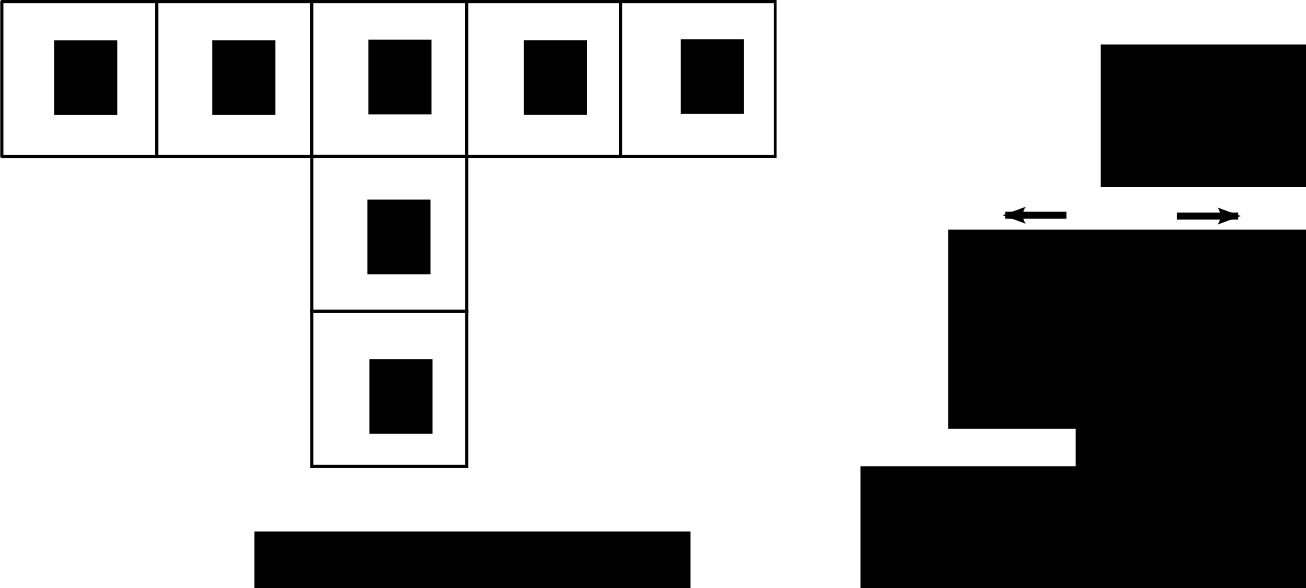
\includegraphics[width=\tworldsize\columnwidth]{\visualspdf/worlds_and_datasets/Tworld_with_state_number_and_action.pdf}
  \caption{The T world and the available actions.}
  \label{fig:Tworld}
\end{figure}

A simulated teacher wants the robot to reach, and stay at, the left edge of the T world (i.e. state 1). To this end, the teacher provides feedback information to the robot. Feedback signals are represented as two dimensional feature vectors and can have two different meanings: ``correct'' or ``incorrect''. As depicted in Figure~\ref{fig:feedbacksignals}, we assume these signals are randomly generated by two multivariate normal distributions, one for each meaning. We associate green and red colors respectively to signals of ``correct'' and ``incorrect'' meanings. When the teacher wants to send a feedback of meaning ``correct'', he samples a signal from the right, green, Gaussian. Respectively, a signal of meaning ``incorrect'' will be generated on the left side of the feature space. These signals are represented in a two dimensional feature space, which could represent any modality used by the teacher to communicate with the robot, such as speech, gestures, facial expression, or even brain signals.

\begin{figure}[!htbp]
  \centering
  \includegraphics[width=\signalwidth\columnwidth]{\visualspdf/worlds_and_datasets/feedback_signals_color.pdf}
  \caption{The feedback signals used in our visual examples. A signal of meaning ``correct'' will be generated on the right side of the feature space, and a signal of meaning ``incorrect'' will be generated on the left side. Importantly, the agent will never have access to the label information, represented by the color of each signal.}
  \label{fig:feedbacksignals}
\end{figure}

The interaction between the agent and the teacher is turn-taking. First, the agent, which is in a particular state, performs one action and transitions to its next state. The teacher is observing the robot and evaluates the robot's actions with respect to the task he has in mind (i.e. the robot should go and stay in state 1). The teacher then sends the corresponding signal to the robot. However, the robot neither has access to the task the user has in mind, nor it has access to the meaning of the signal sent by the teacher. For the sake of the example, we assume that there are only two possible tasks, reaching G1 or G2.

For example, as depicted in Figure~\ref{fig:TworldOneStepUnlabeled}, the agent starts in state 3, performs action left, and ends-up in state 2. The teacher wants the agent to go to G1, therefore he sends a signal of meaning ``correct'' (i.e. in the right part of the feature space). Note that the signal shown in Figure~\ref{fig:TworldOneStepUnlabeled} (left) is neither green or red, its label is undefined.

\begin{figure}[!htbp]
  \centering
  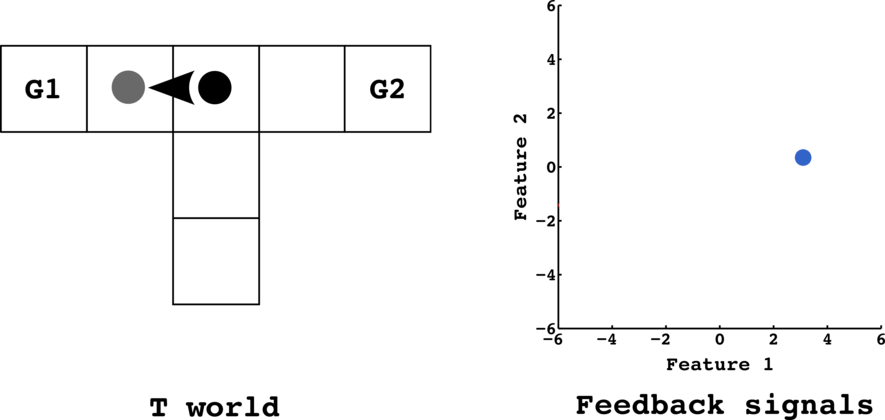
\includegraphics[width=\tworldsize\columnwidth]{\visualspdf/tuto_feedback/Tworld_feedback_unlabeled_one_action.pdf}
  \caption{The teacher provides a feedback signal after each action of the agent. The agent starts in state 3, performs action left, and ends-up in state 2. The teacher wants the agent to go to G1, therefore he sends a signal meaning that the previous action was ``correct'' with respect to the goal. Note that the signal is on the right side of the space as described in Figure~\ref{fig:feedbacksignals}. However the agent does not have access to the label associated to this signal and it only observes a point in a two dimensional space.}
  \label{fig:TworldOneStepUnlabeled}
\end{figure}

After performing many actions randomly, the robot ends-up with a lot of observations associating a state, an action and a feedback signal. As depicted in Figure~\ref{fig:TworldManyStepUnlabeled}, we can observe that two clusters have emerged in the feature space. A straight forward assumption is that one cluster is associated to the ``correct'' meaning, and the other to the ``incorrect'' meaning. We will see how this assumption of consistency in the signals can be exploited in the coming sections.

\begin{figure}[!htbp]
  \centering
  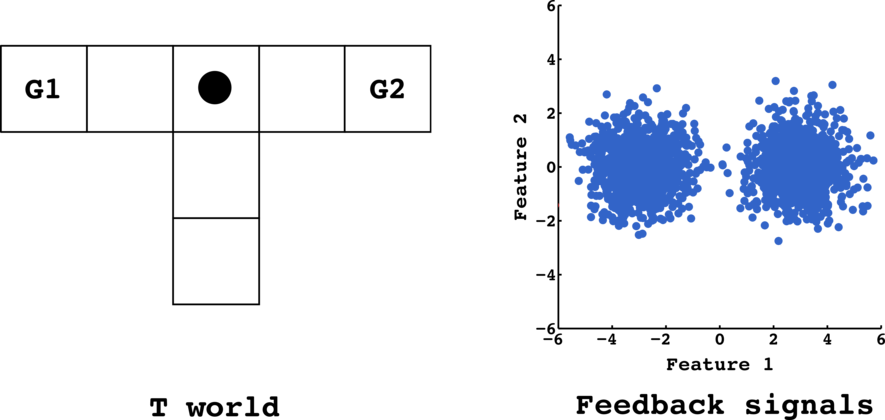
\includegraphics[width=\tworldsize\columnwidth]{\visualspdf/tuto_feedback/Tworld_feedback_unlabeled.pdf}
  \caption{After performing many random actions, the robot ends-up with many of observation associating a state, an action and a feedback signal. The robot does not have access to the label associated to the teaching signals.}
  \label{fig:TworldManyStepUnlabeled}
\end{figure}

\subsection{What the agent knows}

The problem described in this section is impossible to solve without further information. Indeed, even if the agent was able to identify the two clusters, it does not have access to the meaning associated with each cluster. In practice it would be easier if the robot had access to the mapping between teaching signals and their meanings. A typical solution is therefore to rely on a phase of calibration, where the system is given signal-meaning pairs and learns the mapping using a supervised learning algorithm. Given this information, in our example of Figure~\ref{fig:TworldOneStepUnlabeled}, it becomes trivial to identify the task. Starting in state 3, if the robot do action ``left'', it ends up in state 2, and if it receives a signal of meaning ``correct'', then the correct task is to reach the left edge of the T marked by G1.

As mentioned before, in this work the robot cannot rely on the phase of calibration. However the robot has access to the interaction frame, which provide theoretical information about the human teaching behavior. The robot knows:
\begin{itemize}

\item \textbf{Details and timing of the interaction.} After each action, the robot waits for a signal from the teacher. This signal provide information related with the action the robot just performed.

\item \textbf{The set of possible meanings the human can refer to.} The teacher assesses the last action of the robot with respect to an unknown task. The signals' meanings can be ``correct'' or ``incorrect''.

\item \textbf{Constraints on the possible tasks.} There is only two possible tasks, reaching the left (G1) or the right (G2) edge of the T world.

\end{itemize}

In addition the robot has access to the $Frame(Context,Task)$ function that, given a context of interaction and a task, returns the meaning intended by the teacher. For example, the robot knows that if it moves from state 3 to state 2, and that the human wants it to go in G1, then the signals received from the human means ``correct''.
%
\begin{eqnarray}
``correct" = Frame((s3 \rightarrow s2), G1) \nonumber
\end{eqnarray}
%
Respectively, if the robot moves from state 3 to state 2, and that the human wants it to go in G2, then the signals received from the human means ``incorrect''.
%
\begin{eqnarray}
``incorrect" = Frame((s3 \rightarrow s2), G2) \nonumber
\end{eqnarray}

% \subsection{Learning from unlabeled interaction frame}

% In previous chapter~\ref{chapter:humanexperiment:frames}, we defined the terms of interaction frames which represents a stereotyped situations, a schema of interpretation given a particular situation or event. Such frame is often assumed to be known by both the human and the robot in addition to the signal-to-meaning classifier that translate the actual human signals into meaningful symbols. By comparing what the frame predicts and what the human actually said the robot can change our understanding of the situation.

% Learning from unlabeled interaction frames correspond to the problem where the signal-to-meaning classifier is not given, and therefore the robot can not rely on a direct comparison between the prediction from the interaction frame and the observation from the human teacher.

% What remains is the frame. It is at the core of our approach, it is assumed to be known by both the human and the robot. It includes both the constraints related to the task, e.g. teaching a robot which state to reach among a finite set of states, and the protocol used by the teacher to communicate to the robot, e.g. the teacher is assessing the robot's actions. Therefore, the meanings of the unlabeled signals is not explicitly given but is known to belong to a finite set of possible meanings.

% We define a generic frame function that, given a context of interaction and a task, returns the meaning intended by the teacher:
% %
% \begin{eqnarray}
% Meaning = Frame(Context, Task)
% \end{eqnarray}
% %
% Following our previous example, stating that if the robot moves from state 3 to state 4 (context), and that the human wants it to go in G1 (task), then the signals received from the human means ``incorrect'' (meaning), we can exemplify the use of the frame:
% %
% \begin{eqnarray}
% ``incorrect" = Frame((s3 \rightarrow s4), G1)
% \end{eqnarray}

% \transition

% The idea of unlabeled interaction frame summarizes the problem of interaction we tackle in this work. However it is a quite general concept, and in order to understand the underlying principles of our algorithm, in the following sections we will restrict our analysis to simple frames and simple worlds. We will also explicit a number of assumptions related to this work.


%%%%%%%%%%%%%%%%%%%%%%%%%%%%%%%%%%%%%%%%%%%%%%
%%%%%%%%%%%%%%%%%%%%%%%%%%%%%%%%%%%%%%%%%%%%%%
%%%%%%%%%%%%%%%%%%%%%%%%%%%%%%%%%%%%%%%%%%%%%%
%%%%%%%%%%%%%%%%%%%%%%%%%%%%%%%%%%%%%%%%%%%%%%
%%%%%%%%%%%%%%%%%%%%%%%%%%%%%%%%%%%%%%%%%%%%%%
\section{What do we exploit}

% Following our T world example, the robot knowns the world, the effect of it actions. The robot also knows the human wants it to reach one of the two edges of the T world marked with G1 and G2. The robot is also aware of the interaction frame, in our case that the teacher will provide, for each action performed by the robot, a feedback signal meaning either ``correct'' or ``incorrect''. The robot further knows how the teacher should behave with respect to one particular goal.
% Central to our method is a system of hypothesis. 

Following our T world example, we now present a visual representations of the interpretation hypothesis mechanism. From the observation made in chapter~\ref{chapter:humanexperiment:interpretationhypothesis}, the robot will generate interpretation hypothesis of the signals with respect to all possible tasks. For a particular task hypothesis, the robot will assign hypothetic meanings, or labels, to the human signals according to its previous actions and knowing their are either ``correct'' or ``incorrect''. The system is ``reasoning'' as follow: \textit{``If the human wants me to solve task G1, then when I performed action ``left'' in state $3$, its feedback signal should mean ``correct'' ''}. For the sake of our example, we only consider two hypothesis, G1 and G2, as depicted in Figure~\ref{fig:TworldManyStepUnlabeled}.

% We exemplify the idea of interpretation hypothesis following our T world example in section~\ref{chapter:lfui:example}. 

\subsection{Interpretation hypothesis}
\label{chapter:lfui:interpreation}

% We considerer the same interaction as in section~\ref{chapter:lfui:example}. 

% For the sake of the example and ease of explanation, we consider those two-dimensional signals as representing speech utterances.

For each action, the robot receives raw unlabeled two dimensional signals. Following the above explanation, for a particular hypothesis (G1 or G2), the robot can assign hypothetic meanings to the human signals knowing their are limited to a finite set and according to the interaction history. We assume our teacher is optimal and therefore assume our agent is aware of the optimal policies for each task  (see Figure~\ref{fig:Twolrdpolicies}), which can be used to interpret the human signals.

% The machine is ``reasoning'' as follow: \emph{"If the human wants me to solve task G1 then when I performed action $a$ in state $a$ and he said ``oui'', he meant ``incorrect''"}. 

% We exemplify this process using the same example as in Figure~\ref{fig:TworldOneStepUnlabeled} and according to our two task hypothesis which are reaching either of the two edges marked as G1 or G2. 

\begin{figure}[!htbp]
  \centering
  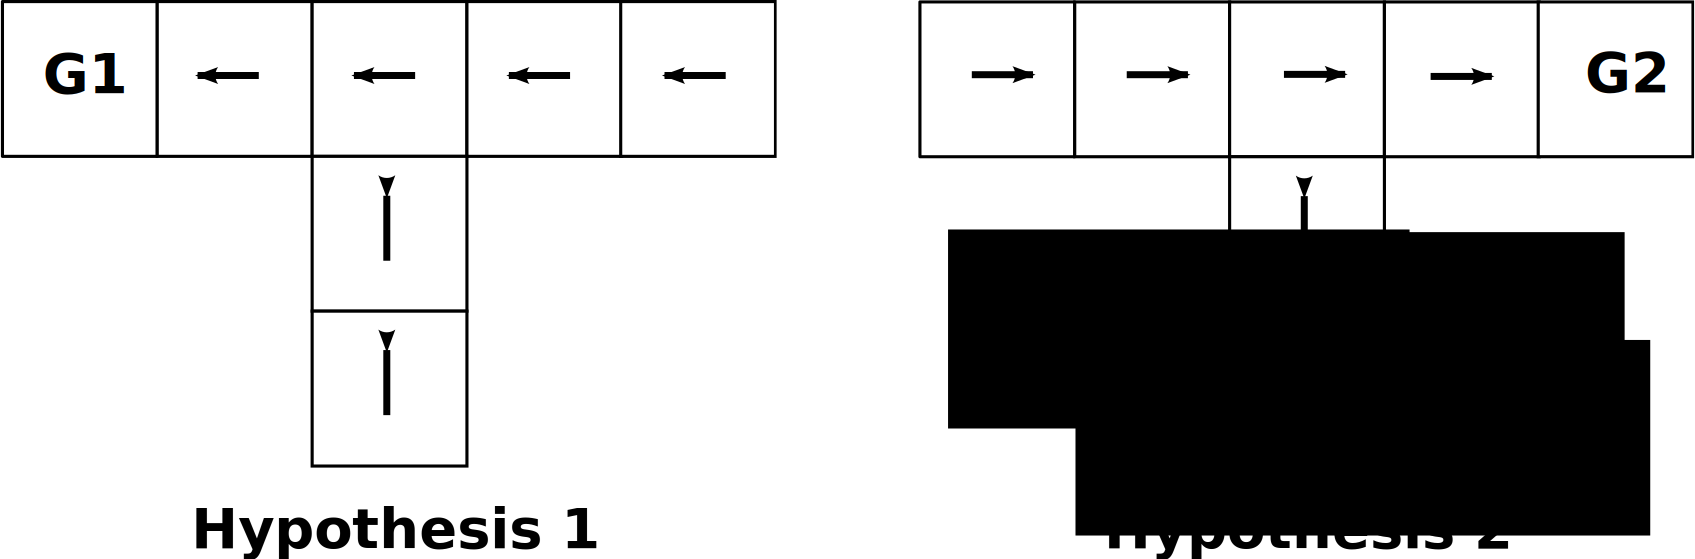
\includegraphics[width=\tworldsize\columnwidth]{\visualspdf/tuto_feedback/Tworld_hypothesis.pdf}
  \caption{Optimal policies associated to the two task hypothesis G1 and G2 in the T world. Such policies are known by both the human and the agent, and allow the agent to interpret a human signal with respect to a given task.}
  \label{fig:Twolrdpolicies}
\end{figure}

The teacher wants the agent to go to G1. The agent starts in state 3, performs action left, and ends-up in state 2. The teacher sends a signal in the right part of the feature space, meaning that the previous action was ``correct''. However the agent does not have access to the label associated to this signal and it only observes a point in a two dimensional space (Figure~\ref{fig:TworldLabelunknown}). The agent generates interpretation hypothesis according to G1 and G2. With respect to G1, the action was ``correct'' (Figure~\ref{fig:TworldLabelG1}), while with respect to G2 the action was ``incorrect'' (Figure~\ref{fig:TworldLabelG1}).

\begin{figure}[!htbp]
    \centering
    \begin{subfigure}[b]{\tworldsize\columnwidth}
        \centering
        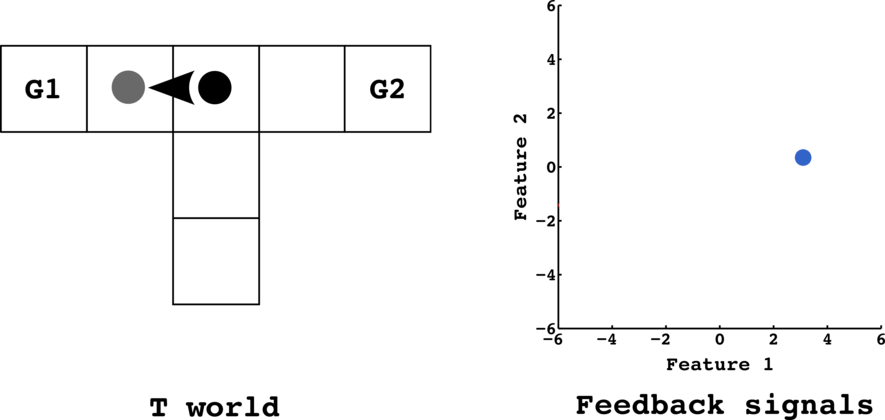
\includegraphics[width=\columnwidth]{\visualspdf/tuto_feedback/Tworld_feedback_unlabeled_one_action.pdf}
        \caption{Feedback signal as received by the agent without label.}
        \label{fig:TworldLabelunknown}
    \end{subfigure}\\
    \begin{subfigure}[b]{\tworldsize\columnwidth}
        \centering
        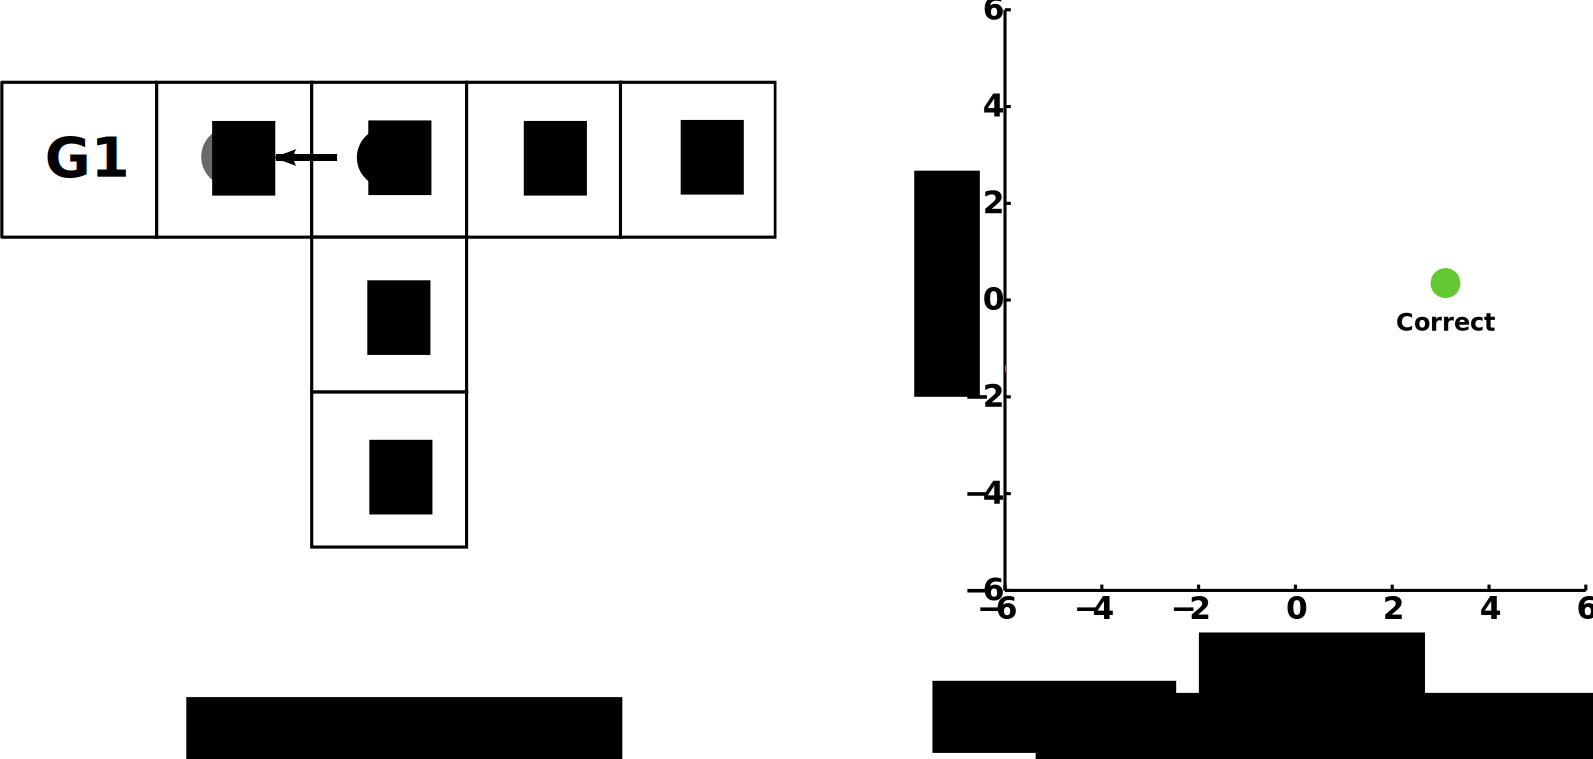
\includegraphics[width=\columnwidth]{\visualspdf/tuto_feedback/Tworld_feedback_labeled_G1.pdf}
        \caption{Feedback signal labeled according to G1.}
        \label{fig:TworldLabelG1}
    \end{subfigure}
    \begin{subfigure}[b]{\tworldsize\columnwidth}
        \centering
        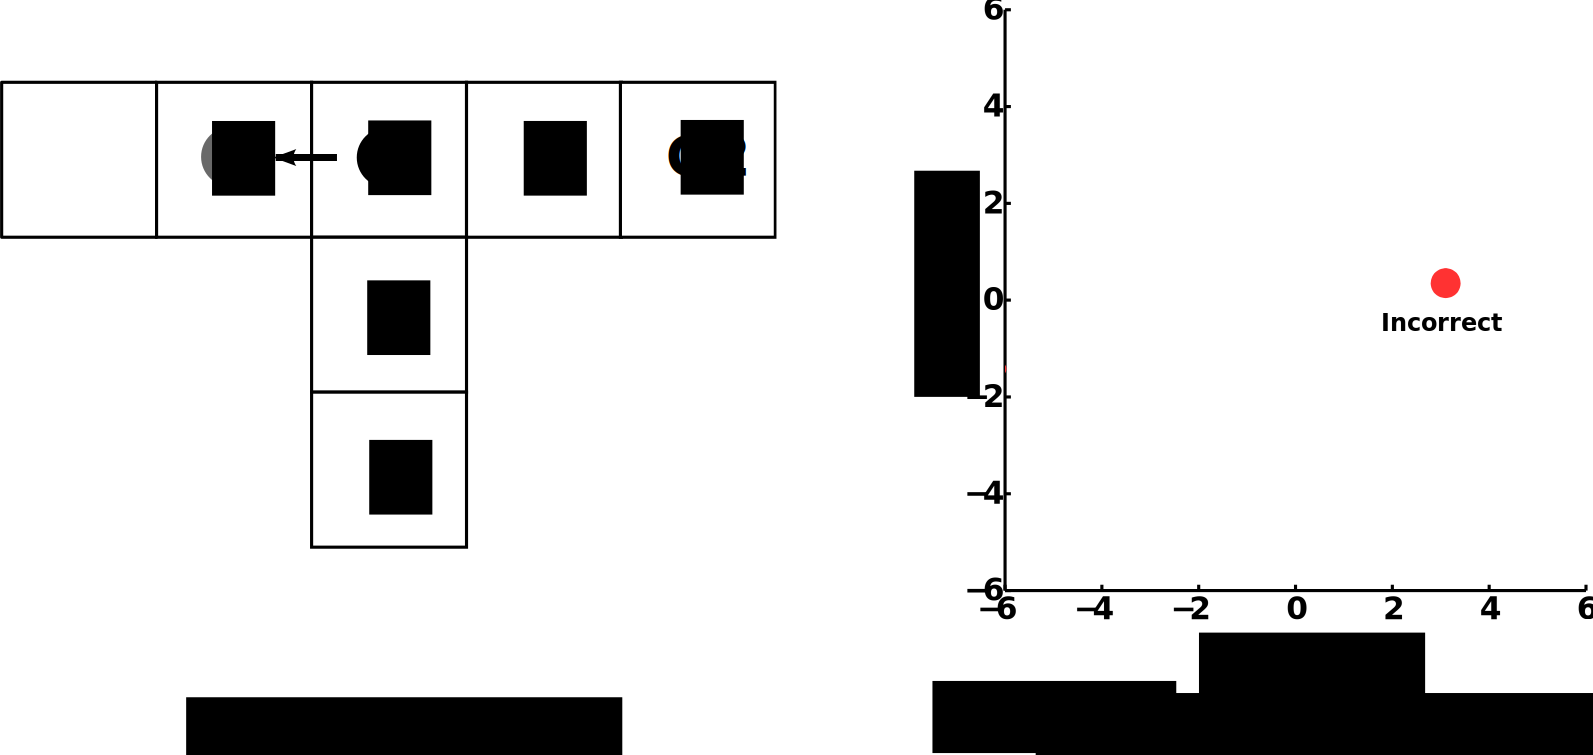
\includegraphics[width=\columnwidth]{\visualspdf/tuto_feedback/Tworld_feedback_labeled_G2.pdf}
        \caption{Feedback signal labeled according to G2.}
        \label{fig:TworldLabelG2}
    \end{subfigure}
    \caption{Interpretation hypothesis made by the agent according to G1 (\ref{fig:TworldLabelG1}) and G2 (\ref{fig:TworldLabelG2}). The agent starts in state 3, performs action left, and ends-up in state 2. The meaning of the signal is different for both hypothesis.}
    \label{fig:TworldLabelOneStep}
\end{figure}

By repeating this process for several iteration steps, with the agent taking random actions and exploring all state-action pairs at least ones, the system end-up with a set of possible interpretation of the human teaching signals (see Figure~\ref{fig:TworldLabelinterpretation}). But as the user has only one objective in mind, in our case G1, only the correct interpretation will assign the correct labels to the observed signals. We say that the corresponding hypothesis exhibit a coherence between the signals and their associated meanings. 

% Note that when the agent moves in the trunk of the T, the interpretation hypothesis with respect to G1 an G2 give the same labels. Details about this interaction will be given in chapter~\ref{chapter:planning} to explain the problem of planning, here we assume the robot explores all state-action.

% \begin{figure}[!htbp]
%     \centering
%     % \begin{subfigure}[t]{\tworldsize\columnwidth}
%     %     \centering
%     %     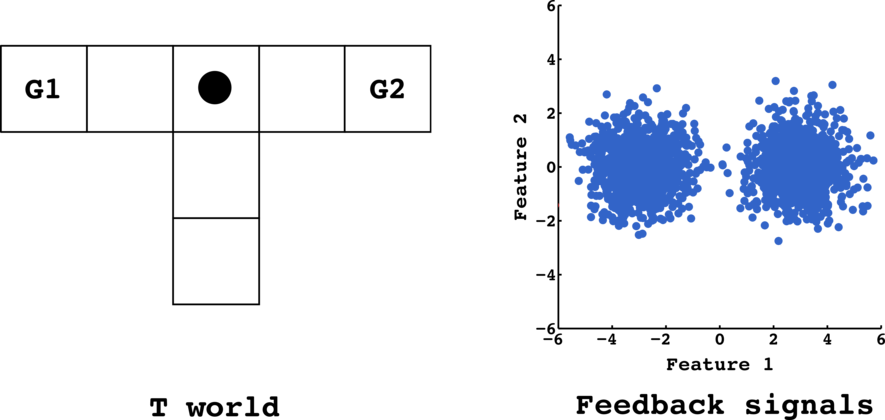
\includegraphics[width=\columnwidth]{\visualspdf/tuto_feedback/Tworld_feedback_unlabeled.pdf}
%     %     \caption{Feedback signals as received by the agent without label.}
%     % \end{subfigure}\\
%     % \begin{subfigure}[b]{\columnwidth}
%         % \centering
%         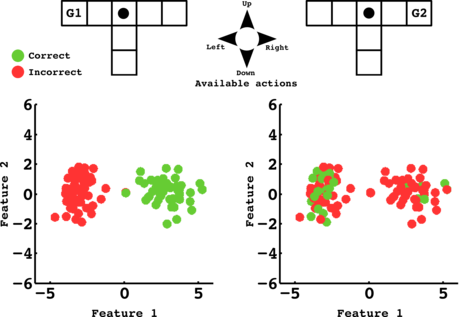
\includegraphics[width=\columnwidth]{\visualspdf/tuto_feedback/Tworld_feedback_labeled_all_actions.pdf}
%         % \caption{Feedback signal labeled according to G1 and G2.}
        
%     % \end{subfigure}
%     \caption{Interpretation hypothesis made by the agent according to G1 and G2 after many interaction steps. The teacher's task is to have the agent reach G1. The agent is exploring all the state space randomly. The labels associated to the task G1 are more coherent with the spacial organization of signals in the feature space.}
%     \label{fig:TworldLabelinterpretation}
%     % \label{fig:TworldLabel}
% \end{figure}

\begin{figure}[!htbp]
    \centering
    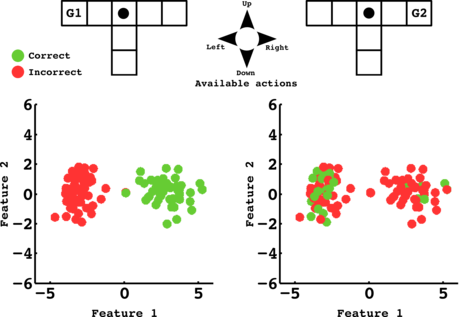
\includegraphics[width=\tworldsize\columnwidth]{\visualspdf/tuto_feedback/Tworld_feedback_labeled_all_actions.pdf}
    \caption{Interpretation hypothesis made by the agent according to G1 and G2 after many interaction steps. The teacher's task is to have the agent reach G1. The agent is exploring all the state space randomly. The labels associated to the task G1 are more coherent with the spacial organization of signals in the feature space.}
    \label{fig:TworldLabelinterpretation}
\end{figure}

Part of the \emph{learning from unlabeled interaction frames} problem defined in chapter~\ref{chapter:introduction:lfui} is the assumption that the user is coherent and uses always the same kind of signal for the same meaning. By visual inspection, we can infer that hypothesis G1 is the correct one as the resulting mapping between signal and meaning is more coherent. The key challenge now is it find out how to identify a coherence between the spacial organization of label in the feature space and their associated labels with the tools available to the robot, i.e. algorithmically. 

We will formalize this idea in section~\ref{chapter:lfui:how}. Before that, we add two comments to this section and we summarize all the underlying assumptions of our problem in section~\ref{chapter:lfui:assumptions}.

\subsection{Different frames}

In our example, we considered only the feedback frames, where the user assesses the robot's actions. In this thesis, we will also consider other interaction frame, such as the guidance frame where the user indicates to the robot which action to perform next. We will provide several visual examples of the guidance frame in the following of this chapter.

% , we simply illustrate here the signal that will be associated to the different action. As depicted in Figure~\ref{fig:guidancesignals}, we used an easy to remember way of presenting the data, the cluster at the top of the feature space represents the ``up'' action, the one at the bottom the ``down'' action, the one at the right the ``right'' action, and the one at the left the ``left'' action.

% \begin{figure}[!htbp]
%   \centering
%   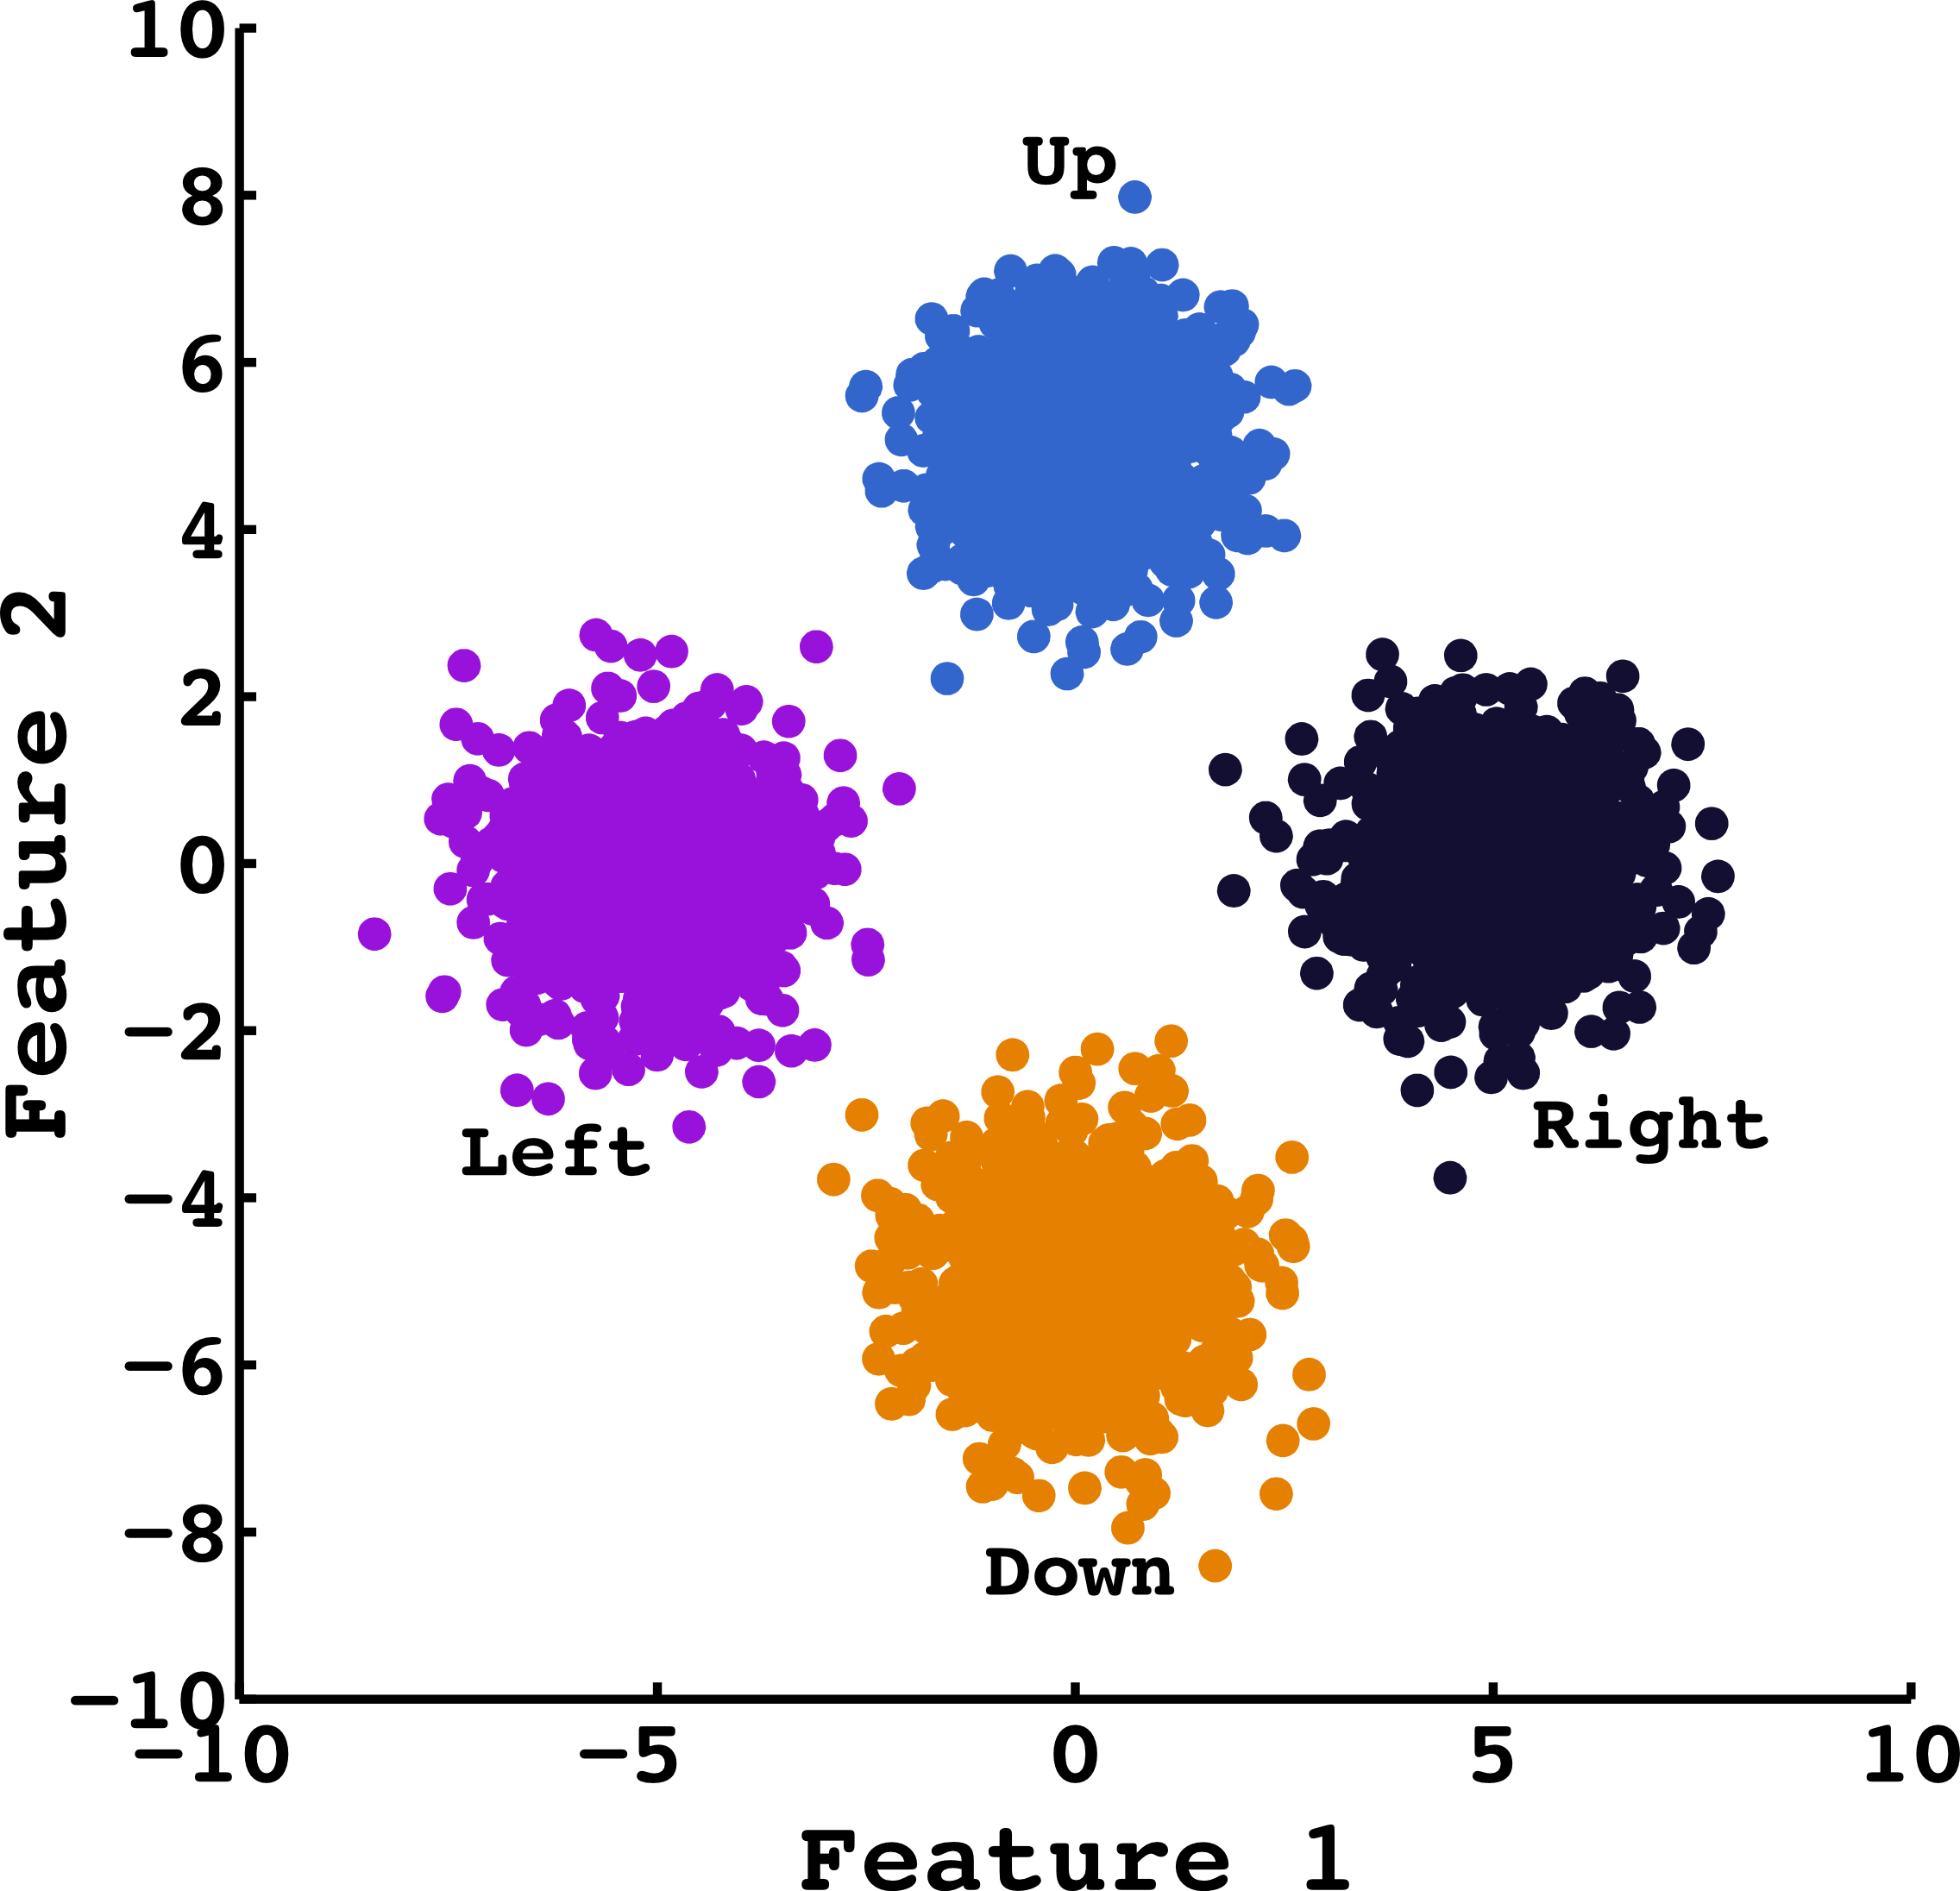
\includegraphics[width=\signalwidth\columnwidth]{\visualspdf/worlds_and_dataset/guidance_4_signals_color.pdf}
%   \caption{The guidance signals used by our simulated teacher in our visual examples.}
%   \label{fig:guidancesignals}
% \end{figure}

\subsection{Why not a clustering algorithm}
\label{chapter:lfui:whynotEM}

When we first look at the unlabeled signals (see Figure~\ref{fig:TworldManyStepUnlabeled}), the first approach that comes to mind is to use a clustering algorithm to identify the two clusters in the feature space. For simple datasets, like the one used in our example, a clustering algorithm will find the two clusters. However, without any additional information, it is impossible to know which one is associated to the meaning ``correct'' or to the meaning ``incorrect''.

More importantly, clustering algorithms are prone to local extrema in the optimization process and for datasets in high dimension with overlapping classes it is unlikely to find the correct underlying structure of the data. Our approach has the advantage to generate hypothetic labels allowing to fit a classifier for each task hypothesis. 

% several empirical results showed that indeed this is the case for data consisting of speech utterances and brain signals.

%%%%%%%%%%%%%%%%%%%%%%%%%%%%%%%%%%%%%%%%%%%%%%
%%%%%%%%%%%%%%%%%%%%%%%%%%%%%%%%%%%%%%%%%%%%%%
%%%%%%%%%%%%%%%%%%%%%%%%%%%%%%%%%%%%%%%%%%%%%%
%%%%%%%%%%%%%%%%%%%%%%%%%%%%%%%%%%%%%%%%%%%%%%
%%%%%%%%%%%%%%%%%%%%%%%%%%%%%%%%%%%%%%%%%%%%%%
\section{Assumptions}
\label{chapter:lfui:assumptions}

As described in the introduction, a number of assumptions are made about the information accessible to the robot and the constraints applied to the interaction. We remind them again briefly here and, now that we have exemplified the mechanism of interpretation hypotheses, we present an additional required property that the world must hold for our problem to be solvable. We will see that, in some cases, it is impossible to discriminate between two hypothesis because they result in symmetric interpretations of the signals. We describe this properties in subsection~\ref{chapter:lfui:symmetries}.

\subsection{Frames}

Our first assumption is that the robot and the human are aware of the frame in which the interaction takes place. This frame regulates the interaction between the two partners, it includes:

\begin{itemize}

\item \textbf{Details and timing of the interaction.} It corresponds to when and how the user will provide instruction signals. For example, the human sends a signal to the robot after every robot's actions. Another example is a human providing a feedback signal between 0.2 and 2 seconds after the robot's action \cite{knox2009interactively}.

\item \textbf{The set of possible meanings the human can refer to.} As depicted before, the set of meaning may include ``correct'' and ``incorrect'' for those cases where the user is assessing the robot's actions. It could also be the set of action names when the user provides guidances on what to do next.

\item \textbf{Constraints on the possible tasks.} The general context of the teaching process is known. For example the robot is aware that the human wants it to reach a specific room in the house, and not to take an object from the fridge. This limits the number of hypotheses the robot can create about what the user has in mind.

\end{itemize}

By combining those three aspects of an interaction frame, the robot can create a set of interpretation hypothesis for the received teaching signals. For one possible task, and given a specific context (e.g. state and action performed in the environment), the robot can infer the meaning intended by the human user ($Meaning = Frame(Context, Task)$). By doing so for every possible task, the agent creates a set of interpretation hypothesis, which we rely on to find the task taught by the user, as well as the signal to meaning mapping.

To do so we rely on specific properties of the human teaching signals.

\subsection{Signals properties}
\label{chapter:lfui:signalproperties}

We make two assumptions about the human teaching signals properties:

\begin{itemize}

\item If the true intended meaning associated to each user signal was known, it would be possible to train a classifier with better than random accuracy. We will see in chapter~\ref{chapter:planning:results} that the performance of the system are highly impacted by the quality of the training data.

\item The teacher is consistent in its use of teaching signals and will always use the name kind of signals to mean the same things. For the case of two buttons, he will always use the same button for the same meaning. It also apply for speech, facial expression, gestures, or brain signals. 

\end{itemize}

Those two properties are typical assumptions in human-robot interaction scenario, we simply assume we can rely on the teacher behavior and that we could, in theory, learn a decoder of the human teaching signals.

However there is one practical constraint that differ from more standard human-robot interaction scenario. Here, in theory, we cannot know in advance if a signal to meaning mapping can be learn. Indeed we do not have access to a database of signal-meaning pairs to train a classifier first, which allow to try different feature extraction processes or different classifiers beforehand. This limitation requires to ensure the representation of the signal as well as the selected classifier allow to learn a usable decoder.

We will see from results in chapter~\ref{chapter:planning:results} that our algorithm can cope with highly overlapping data where the classifier produces close to random prediction.

\subsection{World properties and symmetries}
\label{chapter:lfui:symmetries}

There is some cases where different hypothesis are not distinguishable. As the robot do not have a direct access to the true intended meaning of the teaching signals, it can only rely on the interpretation hypothesis made for each task.

Two problems could appear: \begin{inparaenum}[(a)] \item two hypothesis may share the same interpretation model and cannot be differentiated as they attribute the same meanings to the signals, and \item two hypothesis may end up with opposite interpretations that are both as valid. \end{inparaenum}.

For those cases where two hypothesis share the same interpretation model, either the task are the same with respect the user, either some parts of the problem are hidden to the human, which can not provide appropriate instructions. These questions are the core of the theoretical analysis of Cederborg's thesis \cite{cederborg2014thesis,cederborg2014social}. We do not consider this problematic in this thesis and assume the world properties ensure that two hypothesis will never share the same interpretation model. Most of the hypothesis will share parts of the interpretation model but there will always exist one situation, i.e. one state-action pair, where two interpretation models differs.

For those cases where two hypothesis end up with opposite interpretations that are both valid, we illustrate the problem for the case of both feedback and guidance instructions using a visual example.

\subsubsection*{Symmetries: the feedback case}

We present the line word in Figure~\ref{fig:lineworld} which contains only the top T bar of the T world. This world is well suited to describe the symmetry problem. 

\begin{figure}[!htbp]
  \centering
  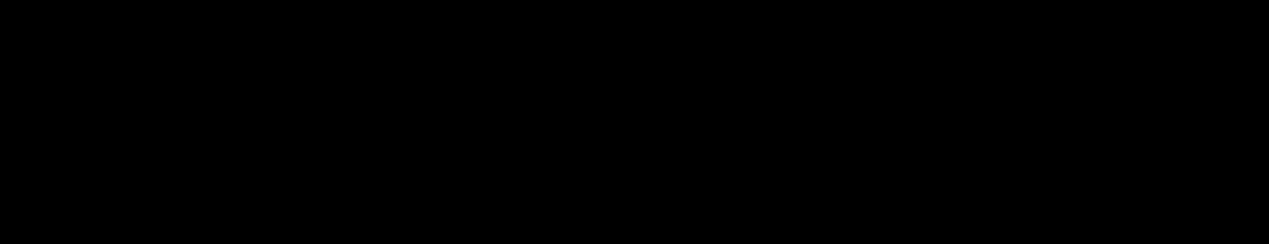
\includegraphics[width=\tworldsize\columnwidth]{\visualspdf/worlds_and_datasets/lineworld_with_state_number_and_2action.pdf}
  \caption{The line world and the available actions.}
  \label{fig:lineworld}
\end{figure}

The interaction follows the same protocol as in previous examples. As depicted in Figure~\ref{fig:lineworldfeedback2action}, after several interaction steps, the interpretation hypothesis for G1 and G2 display symmetric properties. Indeed, according to G1, signals on the left side of the feature space mean ``incorrect'', and signal on the right means ``correct''. Inversely, according G2, signals on the left side of the feature space mean ``correct'', and signal on the right means ``incorrect''. Therefore, even if the interpretation of the signals differ between each hypothesis, the two interpretations are equally coherent. As the optimal policies to reach each of the two goal states are opposite in every state, an action that triggers a ``correct'' feedback with respect to G1, triggers a ``incorrect'' feedback for G2 and vice versa. It is therefore impossible to know the true associated meaning of the signals without further information.

\begin{figure}[!htbp]
  \centering
  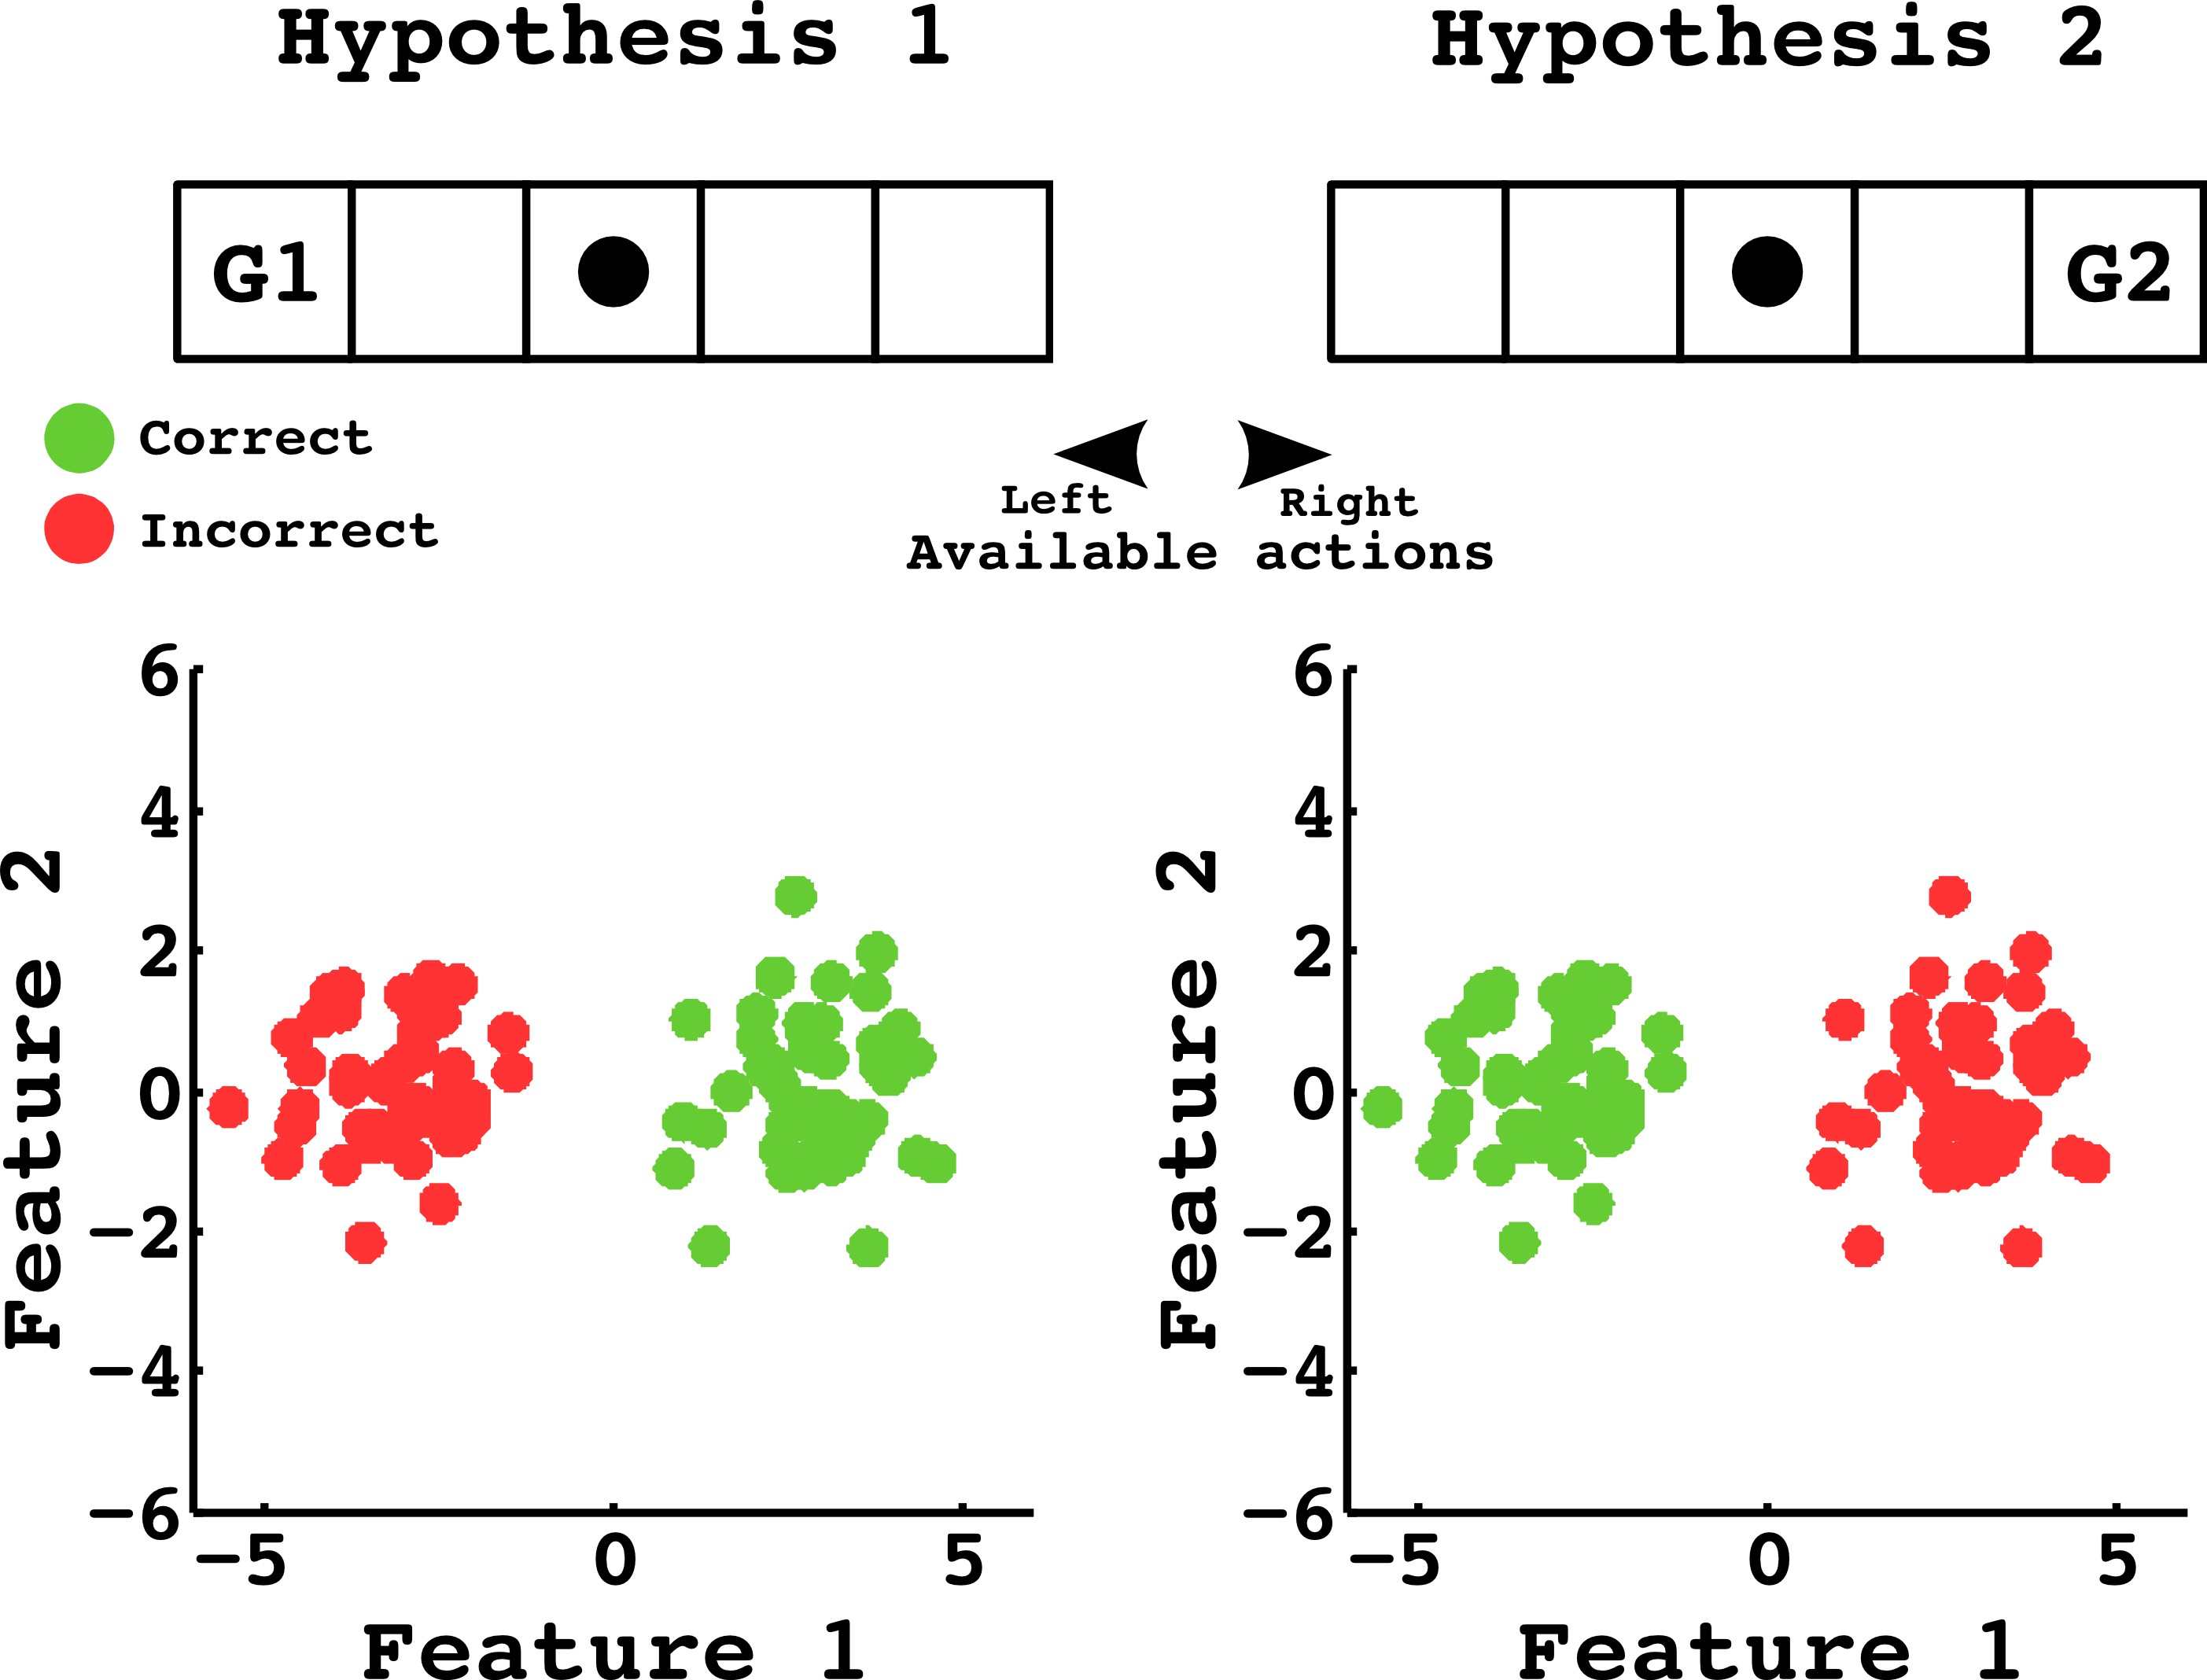
\includegraphics[width=\tworldsize\columnwidth]{\visualspdf/lineworld_symmetries/feedback_2actions.pdf}
  \caption{Interpretation hypotheses made by an agent receiving feedback on its action in the line word and where the hypothetic tasks are G1 or G2. The agent can only perform right or left actions which results in symmetric interpretation hypothesis of the feedback signals.}
  \label{fig:lineworldfeedback2action}
\end{figure}

It is theoretically impossible to differentiate symmetric task hypotheses, therefore we will not consider environments holding this symmetric property. One way to bypass this problem is to add a ``no move'' action, as illustrated in Figure~\ref{fig:lineworld3action}, that is valid only at the goal state

\begin{figure}[!htbp]
  \centering
  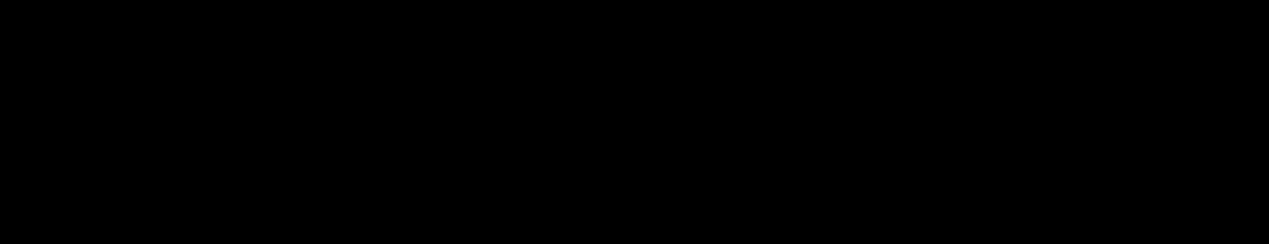
\includegraphics[width=\tworldsize\columnwidth]{\visualspdf/worlds_and_datasets/lineworld_with_state_number_and_action.pdf}
  \caption{The line world and the new available actions, including a ``no move'' action.}
  \label{fig:lineworld3action}
\end{figure}

When taking the ``no move'' action the agent does not change position. This action allow to brake the symmetry effects, as its interpretation will be the same for all states that are not in the set of hypothetic goal state, i.e. all state but G1 and G2. In other words, if the agent performs action ``no move'' in state 3, the user will produce a signal of meaning ``incorrect'' because the agent is not progressing towards the goal state(G1 here). But the agent did not progress either towards the G2. Therefore the signal will be interpreted as ``incorrect'' by the two interpretation hypothesis, breaking the symmetry problem. The interpretation results after several iteration steps, and using the new ``no move'' action, are depicted in Figure~\ref{fig:lineworldfeedback3action}.

\begin{figure}[!htbp]
  \centering
  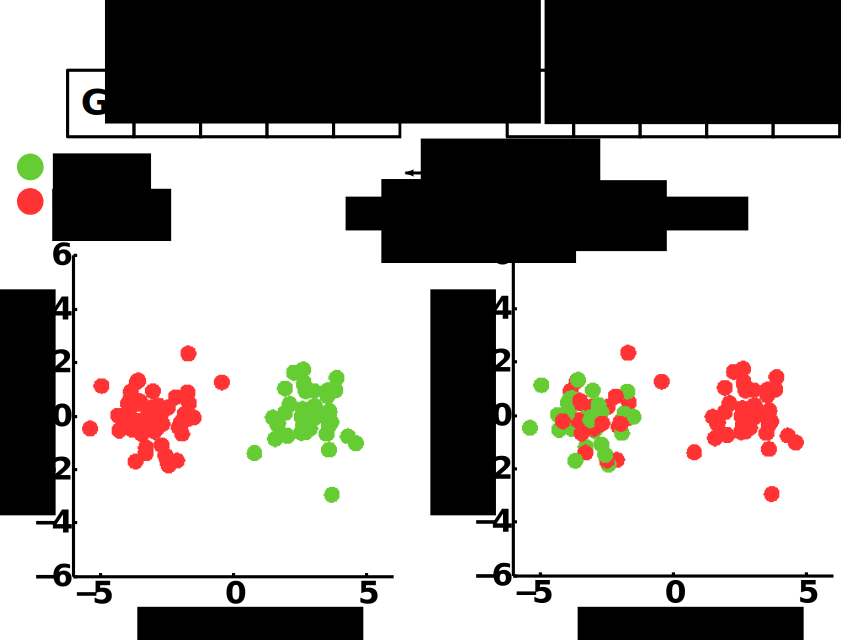
\includegraphics[width=\tworldsize\columnwidth]{\visualspdf/lineworld_symmetries/feedback_3actions.pdf}
  \caption{Interpretation hypotheses made by an agent receiving feedback on its action in the line word and where the hypothetic tasks are G1 or G2. The agent can perform right, left, or ``no move'' actions. As opposed to Figure~\ref{lineworldfeedback2action}, the ``no move'' action allows to break the symmetry of interpretation between G1 and G2.}
  \label{fig:lineworldfeedback3action}
\end{figure}

\subsubsection*{Symmetries: the guidance case}

This problem of symmetries also applies to the guidance frame. Under the guidance frame, the set of possible meaning includes the name of all possible actions. If the agent can only choose between the ``right'' and ``left'' actions, the teacher can only advise for ``left'' and ``right'' actions. We represent the guidance signals from the teacher in a two dimensional feature space as shown in Figure~\ref{fig:lineworldguidance2signals}.

\begin{figure}[!htbp]
  \centering
  \includegraphics[width=\signalwidth\columnwidth]{\visualspdf/worlds_and_datasets/guidance_2_signals_color.pdf}
  \caption{The guidance signals used by our simulated teacher in our line world visual examples with two actions.}
  \label{fig:lineworldguidance2signals}
\end{figure}


We can easily understand that if the teacher can only advise for ``left'' and ``right'' actions, the interpretation hypothesis for G1 will be symmetric as the one for G2. As our user wants the robot to reach G1, it will only produce ``left'' guidance signals, i.e. signals in the left part of the feature space. And the ``right'' commands will never be used. However, these signals will be interpreted as meaning ``left'' according to G1, and ``right'' according to G2. Yet the two interpretation models are equally coherent. The resulting interpretation hypothesis are shown in Figure~\ref{fig:lineworldguidance2action}.

\begin{figure}[!htbp]
  \centering
  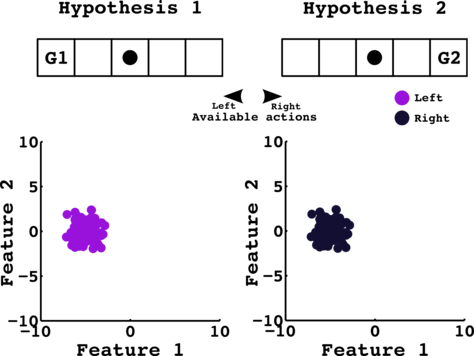
\includegraphics[width=\tworldsize\columnwidth]{\visualspdf/lineworld_symmetries/guidance_2actions.pdf}
  \caption{Interpretation hypotheses made by an agent receiving guidance on its actions in the line word and where the hypothetic tasks are G1 or G2. The agent can only perform right or left actions which results in symmetric interpretation hypothesis of the guidance signals.}
  \label{fig:lineworldguidance2action}
\end{figure}

As for the feedback case, introducing a ``no move action'' allow to break the symmetry. WWith the ``no move'' action available, the user can now produce three different kinds of meaning, which is represented by three different clusters of signals in the feature space (see Figure~\ref{fig:lineworldguidance3signals}). 

\begin{figure}[!htbp]
  \centering
  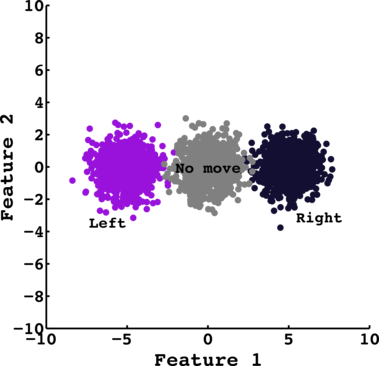
\includegraphics[width=\signalwidth\columnwidth]{\visualspdf/worlds_and_datasets/guidance_3_signals_color.pdf}
  \caption{The guidance signals used by our simulated teacher in our line world visual examples with three actions.}
  \label{fig:lineworldguidance3signals}
\end{figure}

The ``no move'' signal will be used only at the goal state. As this state is not the same for each hypothesis, the ``no move'' signals break the symmetry. The resulting interpretation hypothesis are shown in Figure~\ref{fig:lineworldguidance3action}.

\begin{figure}[!htbp]
  \centering
  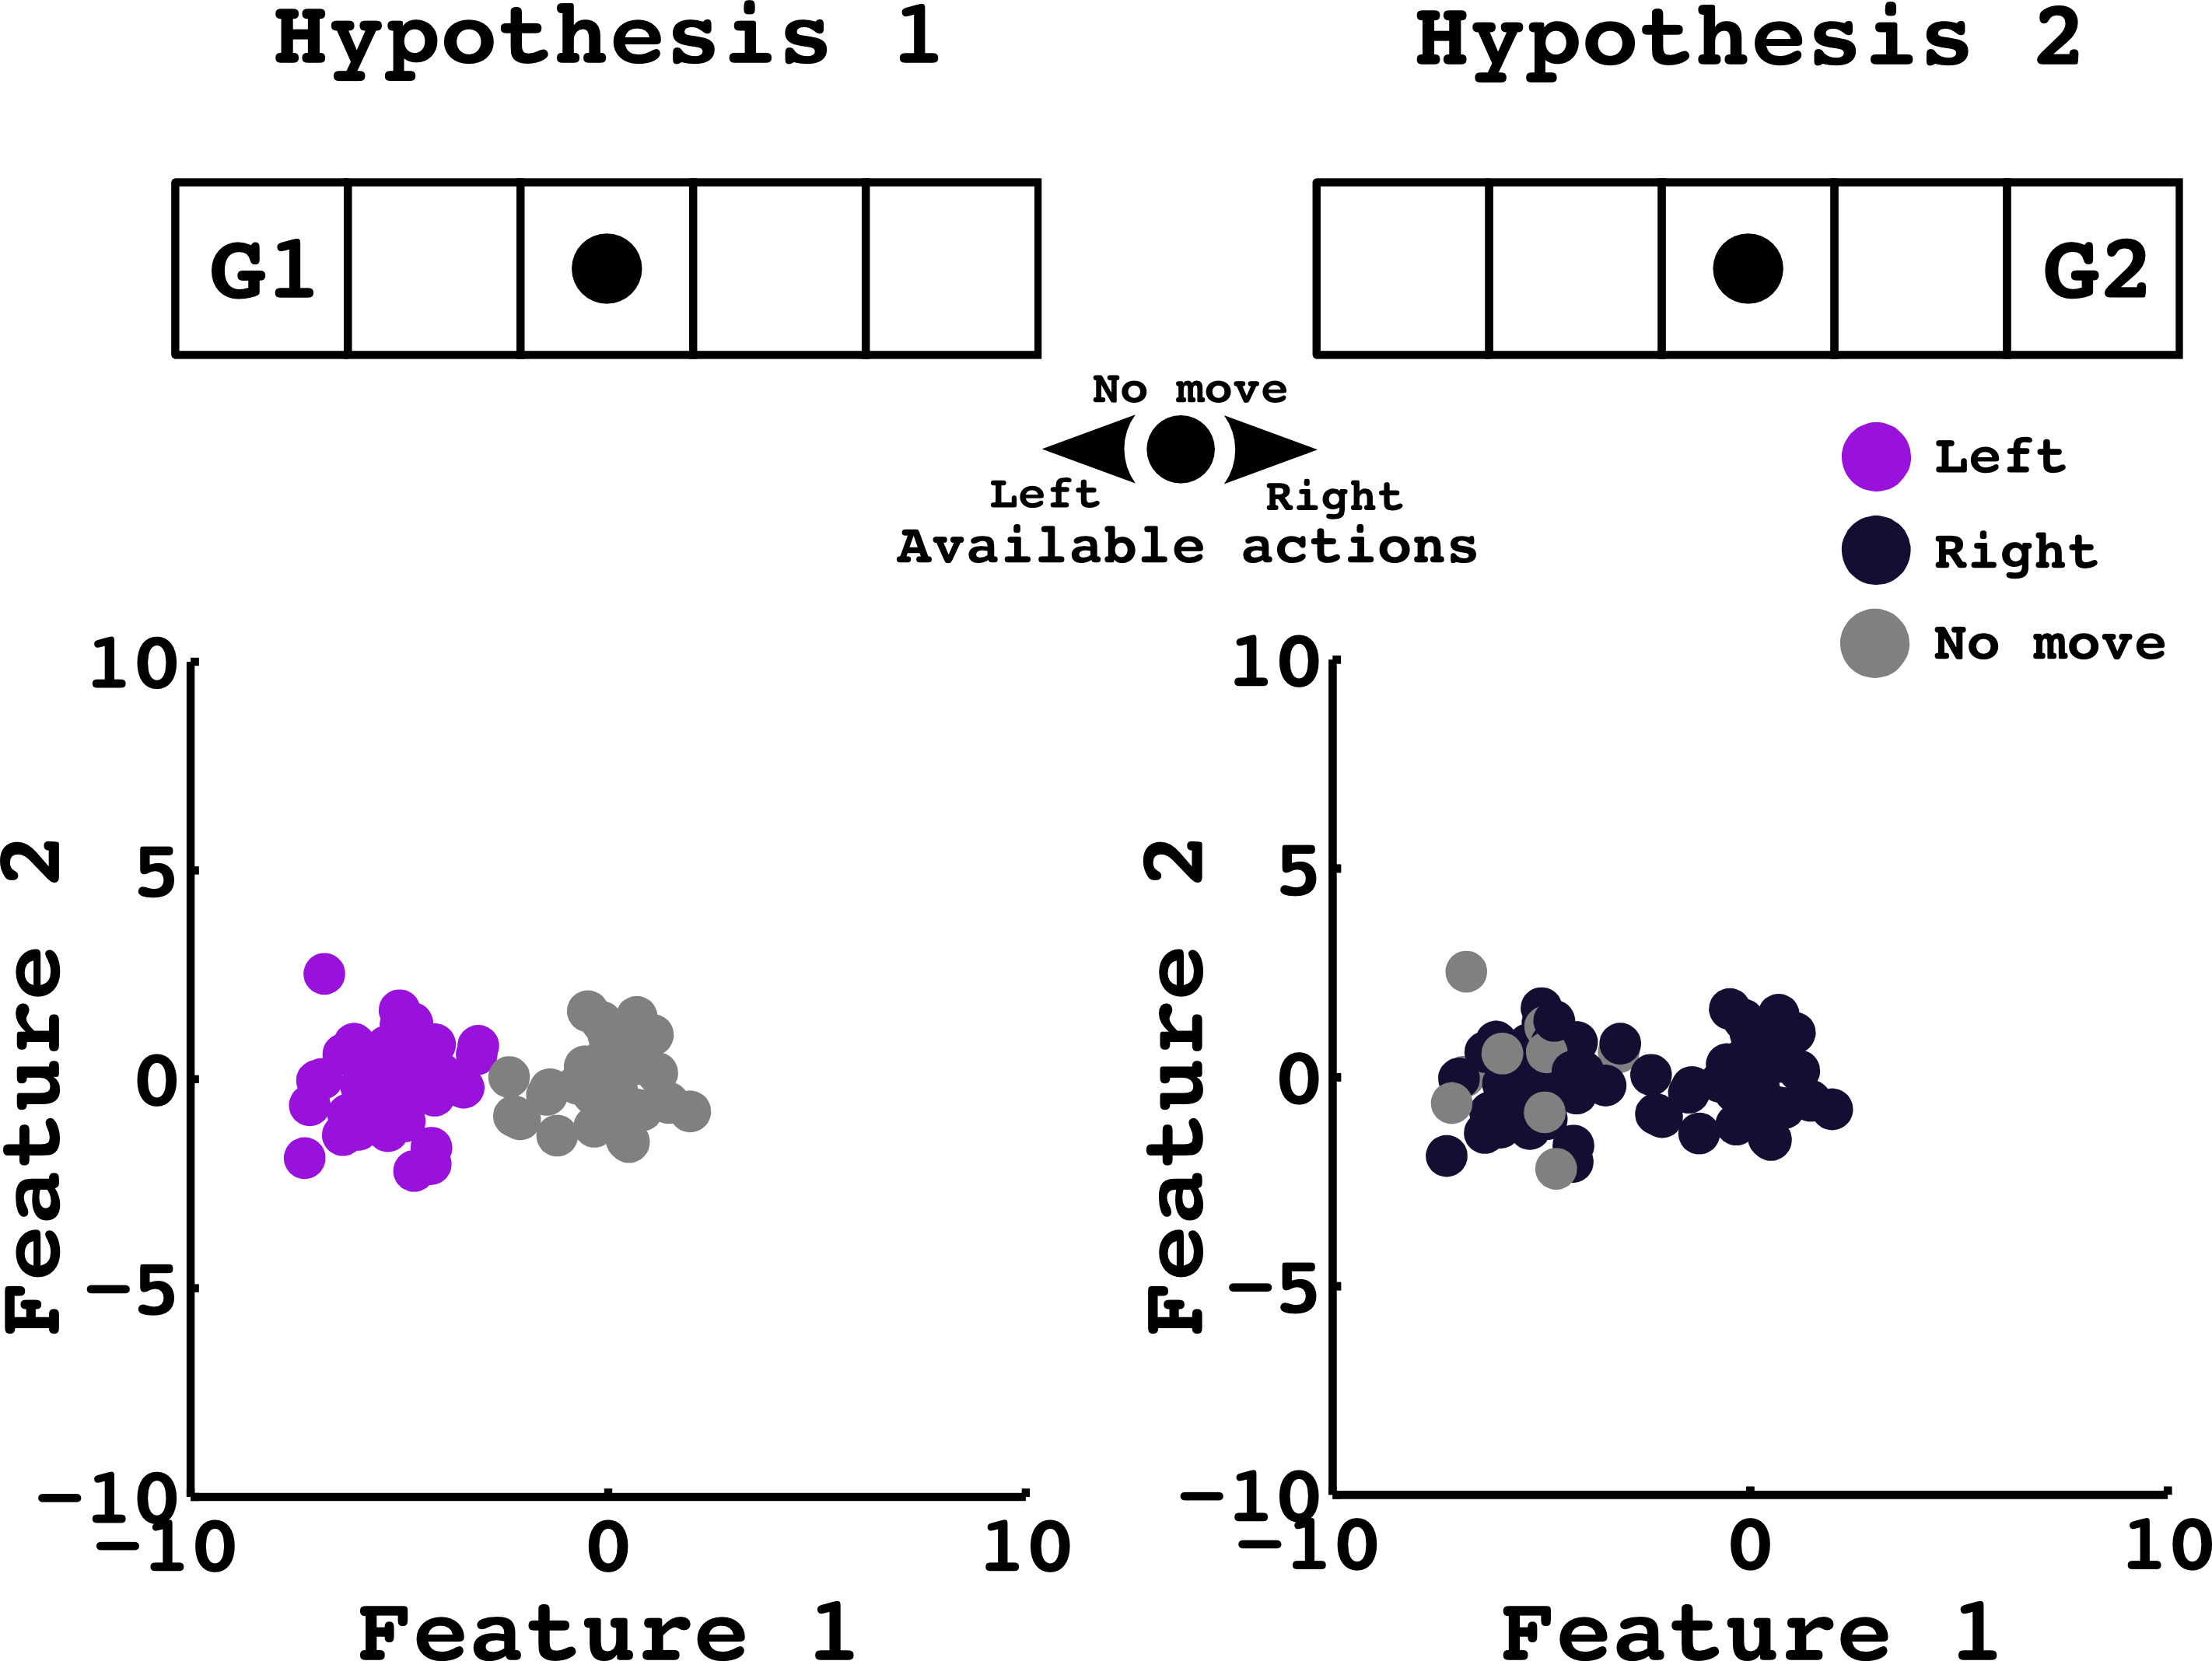
\includegraphics[width=\tworldsize\columnwidth]{\visualspdf/lineworld_symmetries/guidance_3actions.pdf}
  \caption{Interpretation hypotheses made by an agent receiving guidance on its actions in the line word and where the hypothetic tasks are G1 or G2. The agent can perform right, left, or ``no move'' actions. As opposed to Figure~\ref{lineworldguidance2action}, the ``no move'' action allows to break the symmetry of interpretation between G1 and G2.}
  \label{fig:lineworldguidance3action}
\end{figure}

\transition

As it is theoretically impossible to differentiate symmetric task hypotheses, we will not consider environments holding this symmetric property.

\subsection{Robot's abilities}

We further assume the robot is able to plan its action in order to fulfill a specific task. In other words, if the robot knew what the user wants it to do, it will be able to do it. It implies the robot as full knowledge of the world dynamics and knows how to make a plan. This way the robot can understand the theoretical relation between one action, a specific task and a signal of the user; and therefore create interpretation hypothesis.

% However, this ability could have been learn from previous self-exploration session of the environment allowing the robot to learn the dynamics of the environment.

\transition

The following of this chapter will consider the full set of assumptions defined above.

Most of these constraints are typical from interactive learning experiments. Several aspects are often more constrained. Especially, either the signal to meaning mapping is known in advance, and the agent infer the task based on the known instructions \cite{kaplan2002robotic,chernova09jair,knox2009interactively}, either the task itself is known, allowing the robot to assign meanings to the teaching signals such that the signal to meaning mapping can be learned (e.g. the calibration phase for BCI systems). Our method generalize over these approaches as we neither need to know the task, nor the signal-to-meaning mapping.

Other constraints are not always applied, such as the ability of the robot to plan its action, or the fact that a finite number of task is defined in advance.

The ability to plan is linked to the need for the robot to interpret the signals of the user in different situations. To do so the robot needs to be able to project itself in the future to judge of the ``long term'' effects of its actions. 

% It may be possible to considered an agent that is not able to plan its actions. In such cases, the robot should learn first by self-exploration the dynamic of the environment and  infer a plan for a given task.

The finite set of task hypothesis is more of a practical constraint. Considering an infinite set of task hypothesis would add an other layer of complexity. Given our interpretation hypothesis mechanism, we would have to sample a finite number of hypothesis. Then given the results of our hypothesis based method on this finite set, we would have to re-sample some new hypothesis and test them again until some stopping criterion. This sampling process is logically less reliable than assuming the correct task belongs to a finite set. Therefore, in our main experiments, we only consider problems where a finite set of task hypothesis can be defined. It is only in chapter~\ref{chapter:limitations:continuoushypothesis} that this assumption is removed.

%%%%%%%%%%%%%%%%%%%%%%%%%%%%%%%%%%%%%%%%%%%%%%
%%%%%%%%%%%%%%%%%%%%%%%%%%%%%%%%%%%%%%%%%%%%%%
%%%%%%%%%%%%%%%%%%%%%%%%%%%%%%%%%%%%%%%%%%%%%%
%%%%%%%%%%%%%%%%%%%%%%%%%%%%%%%%%%%%%%%%%%%%%%
%%%%%%%%%%%%%%%%%%%%%%%%%%%%%%%%%%%%%%%%%%%%%%
\section{How do we exploit interpretation hypotheses}
\label{chapter:lfui:how}

As exemplified in Figure~\ref{fig:TworldLabelinterpretation}, generating interpretation hypothesis for each possible task allows to find out the task the user has in mind. As the user has only one objective in mind, only the correct hypothesis will assign the correct meanings to the observed signals. In our example, we can identify this task visually, by looking at the coherence between the spacial organization of the signals and their associated meanings. But our robots and algorithms cannot use our visual intuition. The key challenge it to find out a measure that can reflect the coherence between the spacial organization of the signals and their associated meanings.

As a measure of coherence we can measure the quality, i.e. the accuracy, of a decoder trained on each hypothetic dataset of signal-label pairs. As for the wrong hypotheses some signals are not associated with their correct meanings, the quality of the resulting classifiers should be worst than the quality of the classifier trained on the correct hypothesis.

For example, if we assume the signals generated by the teacher can be separated by a quadratic curve, and following our T world example (cf. Figure~\ref{fig:TworldLabelinterpretation}), for each task, we can use the quadratic discriminant analysis (QDA) \cite{lachenbruch1975discriminant} approach to fit a classifier on the data. For two classes, this classifier resumes in computing the maximum likelihood for the mean and covariance matrix associated to each labels. The results of this process is illustrated in Figure~\ref{fig:TworldLabelGaussian}.

\begin{figure}[!htbp]
    \centering
    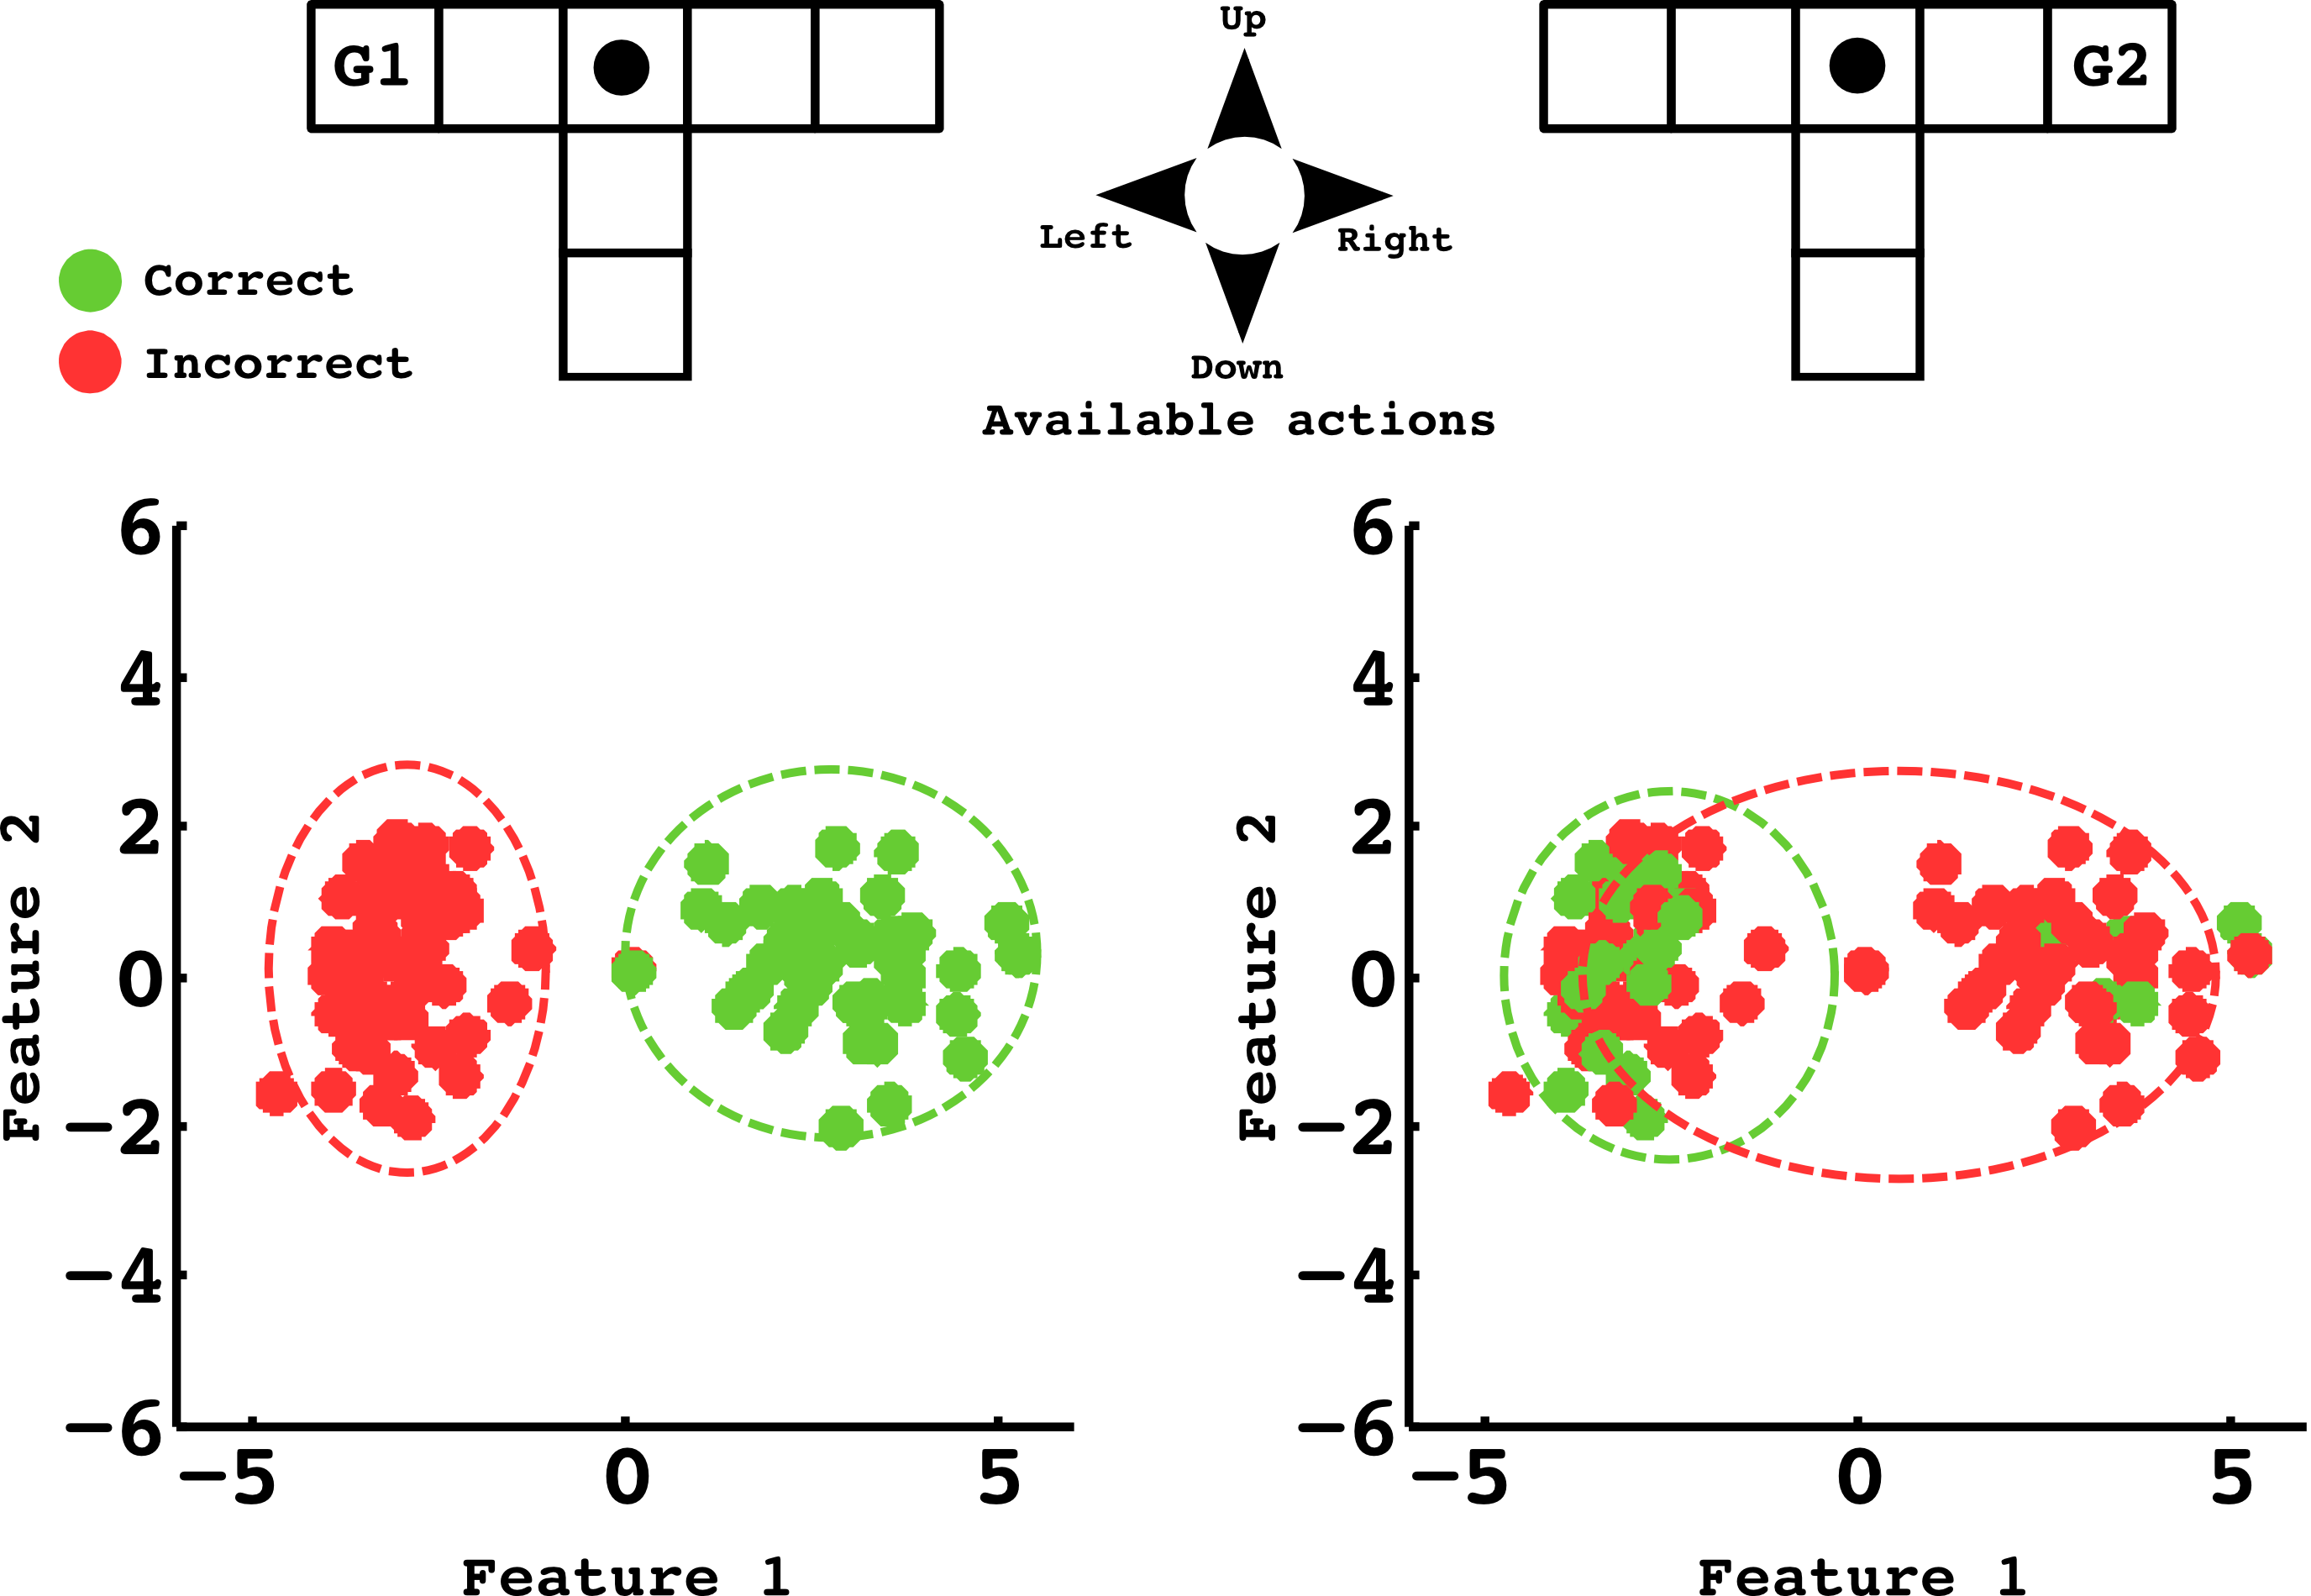
\includegraphics[width=\tworldsize\columnwidth]{\visualspdf/tuto_feedback/Tworld_feedback_labeled_all_actions_with_gaussians.pdf}
    \caption{Interpretation hypotheses made by the agent according to G1 and G2 after many interaction steps. For each class, we compute a Gaussian distribution shown as a dotted line (approximated by hand). The teacher wants the agent to reach G1. The agent is acting randomly. The labels associated to the task G1 are more coherent with the spacial organization of signals in the feature space. It can be measured by the difference in classification performances made by each Gaussian classifier.}
    \label{fig:TworldLabelGaussian}
\end{figure}

By computing the performance of the resulting classifiers, we can test which hypothesis satisfies better the assumption that the signals can be separated by a quadratic curve. As stated in the previous section~\ref{chapter:lfui:signalproperties}, here the choice of the classifier encodes our hypothesis on the underlying structure of the data.

The following of this section formalizes this idea. Next section presents results on a pick and place robotic scenario where the user provides instructions using speech utterances. We use the term label to refer to the meaning associated to user's signals.

\subsection{Notation}

We consider interaction sessions where a machine can perform discrete actions from a set of available actions $a \in \mathcal{A}$ in an either discrete or continuous state space $s \in \mathcal{S}$. The user, that wants to achieve a task $\hat{\xi}$, is providing instructions to the machine using some specific signal $e$, represented as a feature vector  $e \in \mathbf{R}^d$. The task is sequential meaning it is completed by performing a sequence of actions. The machine do not have access to the task the user has in mind, as well as to the actual meaning of each user's signal. Its objective is to simultaneously identify the task and learn to decode user's signals. To achieve this, it has access to a sequence of triplets in the form $D_M = \{(s_i, a_i, e_i),\ i = 1,\ldots,M\}$, where $s_i$, $a_i$ and $e_i$ represent, respectively, the state, action and instruction signals at time step $i$. $D_M$ represents the history of interaction up to step $M$. The behavior of the machine is determined by the actions $a\in\mathcal{A}$ and the corresponding transition model $p(s'\mid s,a)$.

We assume the system has access to a set of task hypothesis $\xi_1,\ldots,\xi_T$ which includes the task $\hat{\xi}$ the user wants to solve. We assume instruction signals $e$ have a finite and discrete number of meanings $l \in \{l_1, l_2, \ldots, l_L\}$ which we call labels. The set of possible labels is known by the machine. We further consider that the agent is given a frame function that given a state $s$, an action $a$ and a task $\xi$ returns a label $l$. We will formalize our algorithm in terms of probabilities, therefore the frame represents the conditional probability of a label given a state, an action, and a task, written as $p(l | s, a, \xi)$.

Given this frame, the history of interaction $D_M$, and the set of possible task $\xi_1,\ldots,\xi_T$, we can generate interpretation hypothesis. For a particular task $\xi$, we can associate a label (or probability of label) to each signal according its associated state and action. For each task, this results is a dataset of signal-label pairs. As there is $T$ task hypothesis, we end up with $T$ hypothetic sets.

We assume that given such one set of signal-label pairs, it is possible to compute one decoder that classifies signals $e$ into labels $l$, which we also call the signal to meaning mapping. The parameters of such a model will be denoted by $\theta$. We formalize the decoder function as the conditional probability of a label given a signal and a set of parameters, written as $p(l|e,\theta)$.

As both the frame and the decoder refers to probabilities of labels, we will use different notation for the labels given by the frame, which we denote $l^f$, and predicted by the classifier, which we denote $l^c$. 

Finally, for a given iteration step $i$, we will subscript our notation with a $i$ referring to the iteration number. $i$ will be the only letter refereeing to iteration numbers. We will abuse notation for labels and $l_i$ will refer to a label at step $i$, e.g. $l^f_i$ is the label given by the frame at iteration $i$. Any other subscripting letter for $l$ will refer to a particular class, e.g. $l_k$ is the $k$ class.

% For each hypothesis, at time $i$, we have several dataset $D_i^{\xi_t}$, which are used to train a classifier parametrize by $\theta_i^{\xi_t}$. Each classifier $\theta_i^{\xi_t}$ represents an interpretation hypothesis of the user given he is trying to instruct the task $\xi_t$.

\subsection{Estimating Tasks Likelihoods}
\label{chapter:lfui:likelihood}

We remind that, to measure the coherence of each interpretation hypothesis, we measure the quality, i.e. the accuracy, of a classifier trained on each hypothetic dataset of signal-label pairs. More precisely, for each interpretation hypothesis, we will compute the probability that every observed signals are correctly classified. We remind that the agent never has access to the true labels of the data, therefore, here, a ``correct'' classification always refers to the hypothetic labels associated to each task.
% In other words, we compute whether or not the classifier computed for the specific state-action pairs is able to separate well the different classes. 

% We assume that the classifier's predictions are independent from the frame's predictions. Therefore t
The probability that one signal is correctly classified is the sum across all labels of the probabilities that a signal is of a given label times the probability that the model classifies it as being of this same label. Given an interaction tuple $(s,a,e)$, a task $\xi$, and a classifier $\theta$, we can compute the probability that the signal $e$ is correctly classified according to the frame as:
%
\begin{eqnarray}
p(l^c = l^f | s, a, e, \theta, \xi) = \sum_{k = 1, \ldots, L} p(l^c = l_k | e, \theta) p(l^f = l_k | s, a, \xi)
\end{eqnarray}
%
where we assume independence between $l^c$ and $l^f$. There exists a dependence between the state-action pair considered $(s,a)$ and the meaning of the signal receive $(e)$, but this relation only exists with respect to the task the user has in mind $\hat{\xi}$, which is unknown to the agent. The role of our algorithm is to identify this task. Therefore when evaluating a signal, our system should not have any a priori about the label of such signal, but only rely on the classifier's prediction.

This equation estimates the joint probability for one iteration step, i.e. given only one interaction tuple $(s,a,e)$, and assuming the classifier is already given. We should now compute the probability that all the labels expected by the frame and all the labels predicted by the classifier match together given the history of interaction and for a hypothesized task. Given the full interaction history $D_M$ up to time step $M$, and a task $\xi_t$, we can infer the expected labels $l^f_{1,\ldots,M, \xi_t}$ associated to the signals $e_{1,\ldots,M}$, and compute the associated classifier represented by the set of parameters $\theta_{M, \xi_t}$.

For clarify, we simplify our notation and remove the $\xi_t$ superscript. It is important for the reader to keep in mind that the robot will never have access to the true intended meaning of the users, therefore, as soon as we infer labels, they are always linked to a hypothesized task. Note that the tuple $(s, a, e)$ are observations independent of the task.

Given the classifier $\theta_M$ associated to the task $\xi_t$ at time step $M$, the probability that every expected and predicted labels match together, which we call the likelihood of the task $\xi_t$, is given by:
%
\begin{eqnarray}
\L(\xi_t) &=& \prod_{i = 1,\ldots,M} p(l^c_i = l^f_i | D_M, \xi_t) \nonumber \\ 
&=& \prod_{i = 1,\ldots,M} \sum_{k = 1, \ldots, L} p(l^c_i = l_k | e_i, \theta_M) p(l^f_i = l_k | s_i, a_i, \xi_t)
\label{eq:matchingoverfitting} 
\end{eqnarray}
%
This equation computes the odds that all the predictions made by the classifier equals the labels used to train this classifier. However, the classifier $\theta_{M}$ is here computed using all the history of interaction including all the pairs $(e_i, l^f_i)$. This is may lead to overfitting problems. For example, if we use a simple nearest neighbor classifier between the provided signal-label pairs, Equation~\ref{eq:matchingoverfitting} will computes a likelihood of 1. Indeed, we train and test on the same dataset. Therefore, we should only estimate the likelihood on signals not used to train the classifier.

What we really want to test is if the system is able to make correct prediction about what the frame will predict for a new, never observed, situation, i.e. a new tuple $(s,a,e)$. One possible option is to incrementally update the likelihood of each task as soon as new data comes in:
%
\begin{eqnarray}
\L_i(\xi_t) &=& p(l^c_i = l^f_i | D_i, \xi_t) ~~ \L_{i-1}(\xi_t) \nonumber \\ 
&=& \left( \sum_{k = 1, \ldots, L} p(l^c_i = l_k | e_i, \theta_{i-1}) p(l^f_i = l_k | s_i, a_i, \xi_t) \right) ~~ \L_{i-1}(\xi_t) 
\label{eq:matchingfilter} 
\end{eqnarray}
%
where $\theta_{i-1}$ is the classifier trained on all the past observations up to time $i-1$ and according to the label generated from task $\xi_t$. And with $\L_{0}(\xi_t)$ being the prior at time 0 (before the experiment start) for the task $\xi_t$, usually uniform over the task distribution.

While this is a good enough option as it will be demonstrated in the remaining of this thesis, it does not use all available information. Indeed, the update that was made at time $i-10$ is now out of date as, at time $i$, we now have $9$ more observation tuples available that may change our classifier. Therefore, it would be better to reassess the performance of the classifier given the full set of observation. To do so, and in order to avoid the problem of overfitting, the classifier should be trained on all data but the one tested. We denote by $\theta_{-i}$ a classifier trained on all data available up to time $M$ but the one of time step $i$. We can now rewrite the likelihood as:
%
\begin{eqnarray}
\L(\xi_t) &=& \prod_{i = 1,\ldots,M} p(l^c_i = l^f_i | D_M, \xi_t) \nonumber \\ 
&=& \prod_{i = 1,\ldots,M} \sum_{k = 1, \ldots, L} p(l^c_i = l_k | e_i, \theta_{-i}) p(l^f_i = l_k | s_i, a_i, \xi_t) 
\label{eq:matching} 
\end{eqnarray}
%
While this equation exhibit minor changes over Equation.~\ref{eq:matchingoverfitting}, it avoids problems of overfitting. However, this Equation quickly becomes computational costly and is unlikely to be usable online in practice. For example, after 100 steps, if just 10 task hypotheses are considered, the system would have to compute 1000 classifiers to update the likelihoods of each task. While for the previous equations (Eq.\ref{eq:matchingoverfitting} and Eq.~\ref{eq:matchingfilter}), if 10 task hypothesis are considered, only 10 classifiers must be computed each step.

Still, this last approach is not taking into account the quality of the classifier itself. The question is of knowing how reliable the prediction of the classifier are. A common method to evaluate the uncertainty on a classifier's predictions is to use a cross-validation procedure to estimate the confusion matrix associated to the classifier. Such confusion matrix allows to infer the conditional probability of one label given the label predicted from the classifier $p(l^{cc} = l_k| l^c = l_q, \theta)$, for every combination of $k$ and $q$ in $1, \ldots, L$. Where $l^{cc}$ is the corrected, or ``temperated'', label predicted by the classifier given our estimates on the quality of the classifier's predictions using the cross validation procedure.

For example, a dummy classifier could predict that any given signal $e$ will have a probability $1$ of being of class $l_1$. This classifier is obviously wrong if there more than two labels in the training dataset, and the cross-validation procedure will capture and quantify the classifier bias. If the training dataset were composed of 2 classes with equal number of samples, the confusion matrix will give us the following information: $p(l^{cc} = l_1| l^c = l_1, \theta) = p(l^{cc} = l_2| l^c = l_1, \theta) = 0.5$. Meaning that when the classifier predicts label $l_1$ there is 50 percent of chances that the true label is $l_1$, and 50 percent that it is actually $l_2$. In other words, the classifier is useless. On the contrary, a perfect classifier, that never makes classification errors will be represented by the following conditional probabilities: $p(l^{cc} = l_1| l^c = l_1, \theta) = p(l^{cc} = l_2| l^c = l_2, \theta) = 1$ and therefore $p(l^{cc} = l_1| l^c = l_2, \theta) = p(l^{cc} = l_2| l^c = l_1, \theta) = 0$.

We include the following measure of uncertainty on the classifier's predictions in Equation~\ref{eq:matching}:
%
\begin{eqnarray}
\L(\xi_t) &=& \prod_{i = 1,\ldots,M} p(l^{cc}_i = l^f_i | D_M, \xi_t) \nonumber \\ 
&=& \prod_{i = 1,\ldots,M} \sum_{k = 1, \ldots, L} p(l^{cc}_i = l_k | e_i, \theta_{-i}) p(l^f_i = l_k | s_i, a_i, \xi_t)
\label{eq:matchingcrossvalidation} 
\end{eqnarray}
%
with:
%
\begin{eqnarray}
p(l^{cc}_i = l_k | e_i, \theta_{-i}) =  \sum_{q = 1, \ldots, L} p(l^{cc}_i = l_k| l^c_i = l_q, \theta_{-i}) p(l^c_i = l_q | e_i, \theta_{-i})
\label{eq:confusion} 
\end{eqnarray}
%
These latter equations capture well the full aspect of the problem. However the computational cost explodes, it would require to train 10000 classifiers after 100 steps, to compute the likelihood of just 10 task hypothesis, and using a 10 fold cross-validation procedure. This is impossible to use in real time and, as for Equation~\ref{eq:matchingfilter}, we will rely on an iterative process to cope with this problem:
%
\begin{eqnarray}
\L_i(\xi_t) &=& p(l^{cc}_i = l^f_i | D_i, \xi_t) ~~ \L_{i-1}(\xi_t) \nonumber \\ 
&=& \sum_{k = 1, \ldots, L} p(l^{cc}_i = l_k | e_i, \theta_{i-1}) p(l^f_i = l_k | s_i, a_i, \xi_t) ~~ \L_{i-1}(\xi_t)
\label{eq:matchingfiltercrossvalidation} 
\end{eqnarray}
%
with:
%
\begin{eqnarray}
p(l^{cc}_i = l_k | e_i, \theta_{i-1}) =  \sum_{q = 1, \ldots, L} p(l^{cc}_i = l_k| l^c_i = l_q, \theta_{i-1}) p(l^c_i = l_q | e_i, \theta_{i-1})
\label{eq:confusionfilter} 
\end{eqnarray}
%
where $\theta_{i-1}$ is the classifier trained on all the past observation up to time $i-1$ and according to the label generated from task $\xi_t$. And with $\L_{0}(\xi_t)$ being the prior at time 0 (before the experiment start) for the task $\xi_t$, usually uniform over the task distribution.

Following this latter equation, at each step, for 10 task hypothesis, and using 10 fold cross-validation to estimate $p(l^{cc} | l^c, \theta_{i-1})$ the system would have to compute 100 classifiers to update the likelihoods of each task.

\transition

To summarize, we described several measures of quality of classifiers. We incrementally included some uncertainty measurements to avoid making too sharp estimates when the classifier are known to be of unreliable and to avoid problems of overfitting.

% (we will use generic name for the task and the classifier parameter, respectively $\xi$ and $\theta$)

Each term of our pseudo-likelihood is computed from three terms: 
\begin{itemize}
\item $p(l^f|s,a,\xi)$ is the frame function, it represents the probability distributions of the meanings according to a task, the executed action and the current state, i.e. it represent the interaction frame. 
\item $p(l^c | e, \theta)$ is the raw prediction of the classifier $\theta$. 
\item $p(l^{cc} | l^c, \theta)$ encodes which label should be actually recovered by $\theta$. It is the probability that the classifier itself is reliable in its predictions. 
% Intuitively, it models the quality of the model $\theta$.
\end{itemize}

In practice our pseudo-likelihood is maximized in two steps. First, the maximum a posteriori estimate $\theta$ of the classifier is computed, and the term $p(l^{cc} | l^c, \theta)$ is approximated using the confusion matrix associated to the classifier based on a cross validation procedure on the training data. Then, given the classifier and the confusion matrix, the likelihood of the task is evaluated. Finally, the best task $\xi$ should be the one that maximizes the pseudo-likelihood.

% It is the probability that the classifier itself is reliable in its prediction.

Note that the term $p(l^{cc} | l^c, \theta)$ is a global approximation of the uncertainty of classifier's prediction. It considers that the classifier suffer from the same biases for any given signal, i.e. it does not depend on the signal $e$ to be predicted.

% predicted signal follow the same ``rule'' and does not depend on the signal $e$ to be predicted.

% A more precise approach would be to consider a confidence measure on the estimation of each point based on the location of this particular point in the feature space, i.e. $p(l^{cc} | l^c, e, \theta)$. For example, a point that is very close to a bunch of point that all belong to the same class is way more likely to be correctly classified than a point far away from any previously seen point or in the middle of a cloud of point with contradictory labels. For example, Montesano et al. in \cite{montesano2012active} use an algorithm that combines beta–binomial distributions and a non-parametric kernel approach to provide the full distribution for the probability of grasping

\subsection{Decision}
\label{chapter:lfui:confidence}

Using any of the measures described above does not inform us about when our system is confident about which task hypothesis is the correct one. Indeed at every iteration step, the likelihood of one task will be higher that all others. Which criteria should we used to decide when ``higher'' is enough?

The simplest method is to normalize the likelihood estimates to $1$, and considered the resulting value as the probability of each task:
%
\begin{eqnarray}
p(\xi_t) = \frac{\L(\xi_t)}{\sum_{u = 1,\ldots, T} \L(\xi_u)}
\label{eq:probanormalize} 
\end{eqnarray}
%
Given this measure, we can define a probability threshold $\beta$, and, when it exists a $t$ such that $p(\xi_t) > \beta$, we can consider the task $\xi_t$ is the one taught by the user.

This method suffers from one important drawback, it does not scale well with the number of hypotheses. Indeed, the more tasks, the more the differences in likelihood between the best task and the other tasks should be important to reach the defined threshold. Consider for example two cases: \begin{inparaenum}[a)] \item for only two tasks whose respective likelihoods are $[0.45, 0.05]$, their normalized likelihood is $[0.9,0.1]$ \item for four tasks whose respective likelihoods are $[0.45, 0.05, 0.05, 0.05]$, their normalized likelihoods are $[0.75, 0.083, 0.0833, 0.083]$. \end{inparaenum}. While the difference of likelihood between the best task and the other tasks is the same in both condition, the normalization decreases the importance of the first task with respect to the others. By scaling this reasoning to one hundred hypotheses, the normalized likelihood method requires immense likelihood differences to reach the same threshold. Therefore, the normalized likelihood method requires to change the threshold for every scenario depending on the number of tasks considered. 

Comparing the likelihood by pairs is a more robust estimate. Considering the example described above, the first hypothesis was 9 times more likely than all other hypotheses in all conditions (2 or 4 tasks considered). We therefore define $W^{\xi_t}$ as the minimum of pairwise normalized likelihood between hypothesis $\xi_t$ and each other hypothesis:
%
\begin{eqnarray}
W^{\xi_t} = \min_{u~\in~{1, \ldots, T} \smallsetminus \{t\}} \frac{\L(\xi_t)}{\L(\xi_t) + \L(\xi_u)}
\label{eq:probapairwise}
\end{eqnarray}
%
When it exists a $t$ such that $W^{\xi_t}$ exceeds a threshold $\beta \in ]0.5,1]$ we consider task $\xi_t$ is the one taught by the user.

Going back to our previous example: \begin{inparaenum}[a)] \item for only two tasks whose respective likelihoods are $[0.45, 0.05]$, their normalized likelihood is $[0.9,0.1]$ while their minimum pairwise normalized likelihood is $[0.9, 0.1]$ \item for four tasks whose respective likelihoods are $[0.45, 0.05, 0.05, 0.05]$, their normalized likelihoods are $[0.75, 0.083, 0.0833, 0.083]$ while their minimum pairwise normalized likelihood is $0.9, 0.1, 0.1, 0.1]$. \end{inparaenum} With our latter measure $W^{\xi_t}$, we can define a threshold that will hold for every scenario independently of the number of hypothesis.

In our various experiments, both measures will be considered.

\subsection{From task to task}
\label{chapter:lfui:tasttotask}

\begin{figure}[!htbp]
  \centering
  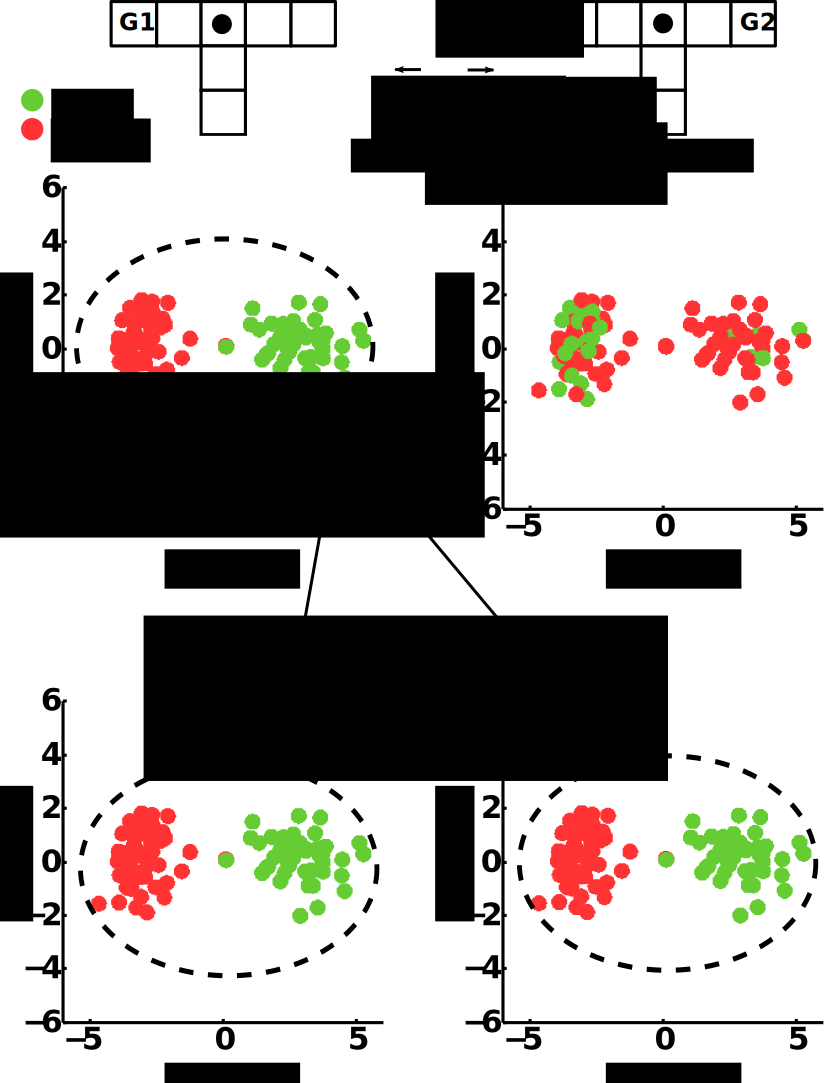
\includegraphics[width=\tworldsize\columnwidth]{\visualspdf/reuse/Tworld_feedback_propagate_labels.pdf}
  \caption{Once a task is identified with confidence, we propagate the labels of the best hypothesis to all the other hypotheses.}
  \label{fig:TworldPropagate}
\end{figure}

Once a task is identified with confidence, the robot executes that task and prepares to receive new instructions from the user according to a new task. Assuming the user starts teaching a new task using the same kind of signals, we now have much more information about the signal to meaning mapping. Indeed, once we are confident that the user was providing instructions related to a specific task, we can infer the true labels of the all the past signals. Therefore we can propagate these labels to all other task interpretation hypothesis (see Figure~\ref{fig:TworldPropagate}), and, by using the same algorithm, we can start learning the new task faster as all hypothesis now share a common set of signal-label pairs. As described in Figure~\ref{fig:TworldReuse}, the signal to meaning models for each hypothesis are still updated every step until the new task is identified and labels reassigned.

\begin{figure}[!htbp]
  \centering
  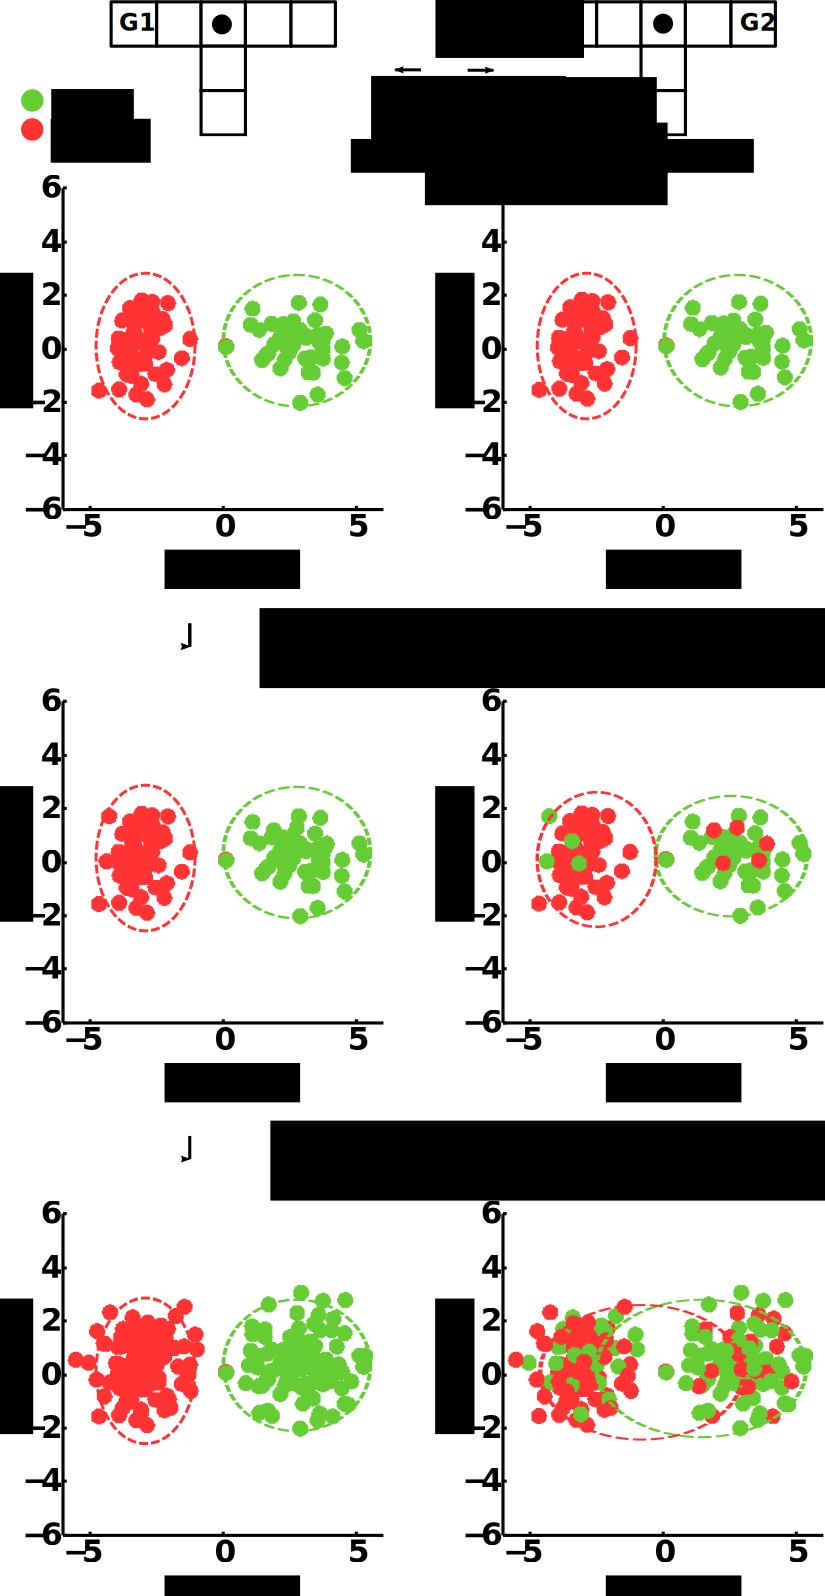
\includegraphics[width=\tworldsize\columnwidth]{\visualspdf/reuse/Tworld_feedback_teaching_again.pdf}
  \caption{When teaching a second task, all hypotheses start with the same signal-label pairs. After a few new interaction steps, some differences in labeling occurs which are easy to detect as they do not conform with the now shared signal model. Therefore allowing to discard quickly the hypothesis G2. We note the interpretation hypothesis process continues to impact the classifiers of each task. The classifier associated to the correct task (here G1) keeps the same quality level, but the one associated to G2 progressively becomes less accurate. This is clearly visible after many steps in the new interaction session.}
  \label{fig:TworldReuse}
\end{figure}

This phase of reuse of previous information could be assimilated to the results of a calibration procedure. Indeed, after a first run we have access to the true intended labels associated to the human signals. The simplest option is therefore to compute one classifier, common all tasks, and to use it to classify new signals.

The method described above differs in that we keep assigning hypothetic labels for each task and we keep updating every classifier. This process allows to decrease the quality of the classifier associated to wrong hypotheses. It helps identifying the correct task faster and more robustly. This effect is more important for the first few task identified. But as the number of signal-label pairs shared between hypothesis increases, the number of new observations needed to sensibly the classifiers increases. Therefore our method progressively converges to the use of a common classifier shared among all hypothesis. This process will be tested in chapter~\ref{chapter:bci} where we will compare our method with a standard calibration procedure approach using EEG signals.

\subsection{Using known signals}
\label{chapter:lfui:known}

In some cases, the robot may already understand some of the communicative signals from the human. For example, the user could have access to two colored buttons, one green to mean ``correct'' and one red to mean ``incorrect''. But the user may prefer using speech to interact with the robot. To allow for flexible interaction, such speech command should not be preprogrammed as each user may speak a different language, or may prefer using the word ``yes'' instead of ``correct'' for example. Considering the mapping between buttons and meanings is known and the mapping between speech utterances and meanings is unknown, we can add a terms to our likelihood equations that includes the information provided by the known signals.

Knowing the meaning of a signal is knowing the parameters $\theta_{button}$ corresponding to the mapping between button presses and their meanings. We can therefore define a separate likelihood update for the known signals, but we simply use the same classifier for each task:
%
\begin{eqnarray}
\L_{button}(\xi_t) &=& \prod_{i = 1,\ldots, M} p(l^{cc}_i = l^f_i | s_i, a_i, e_i, \xi_t, \theta_{button})
\end{eqnarray}
%
The likelihood from the speech can be computed using the equations described in subsection~\ref{chapter:lfui:likelihood}, which we rename $\L_{speech}(\xi_t)$ for convenience.

Finally we can compute the final likelihood as the product of both estimates:
%
\begin{eqnarray}
\L(\xi_t) &=& \L_{button}(\xi_t) ~~ \L_{speech}(\xi_t)
\end{eqnarray}
%
It is important to understand the difference between our approach and a method learning from signals of known meanings. With our approach, we estimate one classifier per task hypothesis. However, if we have access to the true signal to meaning mapping, we must use the corresponding classifier for all hypothesis. Therefore all the equations remain the same, only replacing a global classifier for known signals by hypothetic ones for unknown signals.

\subsection{Summary and rephrasing}
\label{chapter:lfui:rephrasing}

This subsection is meant to re-explain, from a slightly different perspective the ideas and structure behind the different steps of our algorithm. The readers that understand all the aspects of the algorithm can safely skip this subsection.

The algorithm is divided into a classification algorithm, estimating one classifier for each hypothesis based on past interaction, and a filtering algorithm that uses the predictions and properties of this classifier to update a belief over all tasks hypothesis.

The key point is that each hypothesis is considered as if it was the true one. We model the signal to meaning mapping of the user with respect to each task. We then simply test if each classifier can make accurate predictions. As the user is acting according to only one hypothesis, only that hypothesis will be able to predict correctly future interactions.

% Our assumptions is that the hypothesis which show more coherence between expected label and predicted label.

As we have detailed previously, once a task is correctly identified, we have access to the true intended labels of the user. Therefore we should be able to learn a second task faster. We now try to highlight the different processes acting during a full experiment of learning multiple tasks. We will refer to two phases: \begin{inparaenum}[a)] \item phase 1 is learning the first task from unlabeled instructions, and \item phase 2 is learning a second (or third, or \ldots) task knowing we already inferred a first task. \end{inparaenum} Our algorithm is the same for the two phases but different properties are more or less active during phase 1 or phase 2.

Phase 1 is the main contribution of this work. It enables a system to be instructed a new task using signals whose associated meanings are initially unknown. As stated before, our method generates interpretation hypothesis over the possible tasks, infers the hypothetic labels associated to the signals, computes a classifier for each hypothetic set of signal-label pairs, and assumes the one of better quality corresponds to the one the user has in mind. What really have an important impact during phase 1 is not the raw predictions of each classifier, but our measure of uncertainty on their predictions. Indeed, with very few data available, most classifiers are unable to predict correctly unseen data. Even the classifier associated to the correct task might be initially of bad quality, because of the noise in the teaching signals. Therefore all classifiers are considered as unreliable, and our Equation makes only small updates each step. It is only once one classifier stand apart as being more reliable than the others that differences between likelihoods will emerges.

% By doing so the system ends up knowing what is the task taught by the teacher and consequently what are the true labels associated to the teaching signals. Consequently, at the end of phase 1, the system knows a lot more about the mapping between human signals and their meaning.

Phase 2 is almost the contrary. After the first task is correctly identified, we have access to the true labels associated to each signals. One option may be to train a common classifier and consider the teaching as a known source of information. That way learning a second task should be a lot faster as the signal to meaning mapping is known. But this might not be the best option as phase 1 can be quite efficient to identify a first task. For example, as we will see in chapter~\ref{chapter:bci}, it is possible to identify a task in less than 100 iterations using brain signals, while a usual calibration procedure takes around 400 steps. If we stopped after the first task is identified, we could only use 100 signal-label pairs to train a classifier. This classifier is likely to be sub-optimal, making more classification errors. We will indeed observe that a classifier trained on 200 samples makes more errors than one trained on 400 samples.

Our algorithm improves over this approach. After phase 1, we only assign the true labels to all hypothesis. But we keep our hypothesis based approach, as in phase 1, which means we keep updating all the classifiers. Obviously, all classifiers will be very similar, and we maintain similar learning properties than when using a common classifier for each task, i.e. we discriminate the tasks faster. But the key point is that we continue using interpretation hypothesis, generating new signal-label pairs, potentially different for each task. And as wrong hypothesis will add wrong signal-label pairs to their classifiers, the quality of their classifier will also reduce, therefore reducing the sharpness, and quality, of their predictions; which we take into account in our updates. Obviously this effect will be quite small compared to phase 1 because an increasing number of signal-label pairs are shared between hypothesis. But it allows for a smooth transition between the two regimes of our algorithm. Indeed, the more task are identified, the more data are shared between classifiers, and the more signal-label pairs are needed to modify the properties of a classifier. We will see in later experiments with brain signals that the process used in phase 2 reduces the number of mistakes made by the system, especially when the number of teaching signals is still low.

% In the beginning phase 2, all the classifiers are the same, the difference between hypothesis will be on the match between classified signal and expected label. As we interact with the user, some teaching mistake occurs (\textbf{teaching mistake with respect to the hypothesis considered}) that both create non expected prediction from the classifier and decrease the trust I put into my classifier by mixing labels.

To sum up, the same processes and equations are active in both phase. We measure the expected classification performance of each classifiers taking into account the classifier intrinsic quality. In phase 1, it is the classifier intrinsic quality that has the most impact. In phase 2, it is the classification of each individual point that has the most impact. The second phase is actually more of a transition between two regimes of our algorithm. The first regime is phase 1 when very few data are similar among hypothesis. The second regime is comparable to the result of a calibration procedure, it happens once all classifiers are similar and are trained on so much data that a few more signal-labels pairs do not modify their performances. Between these two regimes, there is a phase of transition starting once a first task is identified and the corresponding labels are  transferred to the other tasks.

This detailed analysis of our algorithm should progressively become clearer in the following chapters, especially in chapter~\ref{chapter:bci}.

\transition

In next sections, we present results from our algorithm considering a pick and place robotic scenario where a human wants a robot to build a specific structure with cubes and provides instructions to the robot using vocal commands, whose meaning are unknown to the robot at start. We present results both in simulation and with a real robotic system where we test different aspects: \begin{inparaenum}[(a)] \item how our algorithm scale to a robotic scenario considering a feedback frame, \item how it behaves for the case of guidance words, \item the combining of unlabeled signals with signals of known meanings (buttons), \item the reuse of a learned signal-to-meaning mapping for the learning of a new task. \end{inparaenum}

%%%%%%%%%%%%%%%%%%%%%%%%%%%%%%%%%%%%%%%%%%%%%%
%%%%%%%%%%%%%%%%%%%%%%%%%%%%%%%%%%%%%%%%%%%%%%
%%%%%%%%%%%%%%%%%%%%%%%%%%%%%%%%%%%%%%%%%%%%%%
%%%%%%%%%%%%%%%%%%%%%%%%%%%%%%%%%%%%%%%%%%%%%%
%%%%%%%%%%%%%%%%%%%%%%%%%%%%%%%%%%%%%%%%%%%%%%
\section{Method}

We construct a small size pick-and-place task with a real robot. This robot is going to be programmed using a natural speech interface whose words have an unknown meaning and are \textbf{not} transformed into symbols via a voice recognizer. The robot has a prior knowledge about the distribution of possible tasks.

The interaction between the robot and the human is a turn taking, the robot performs an action and waits for a feedback, or guidance, instruction to continue. This allows to synchronize a speech wave with its corresponding pair of state and action. The experimental protocol is summarized in figure \ref{fig:lfui:bloc}.

\begin{figure}[!htbp]
  \centering
  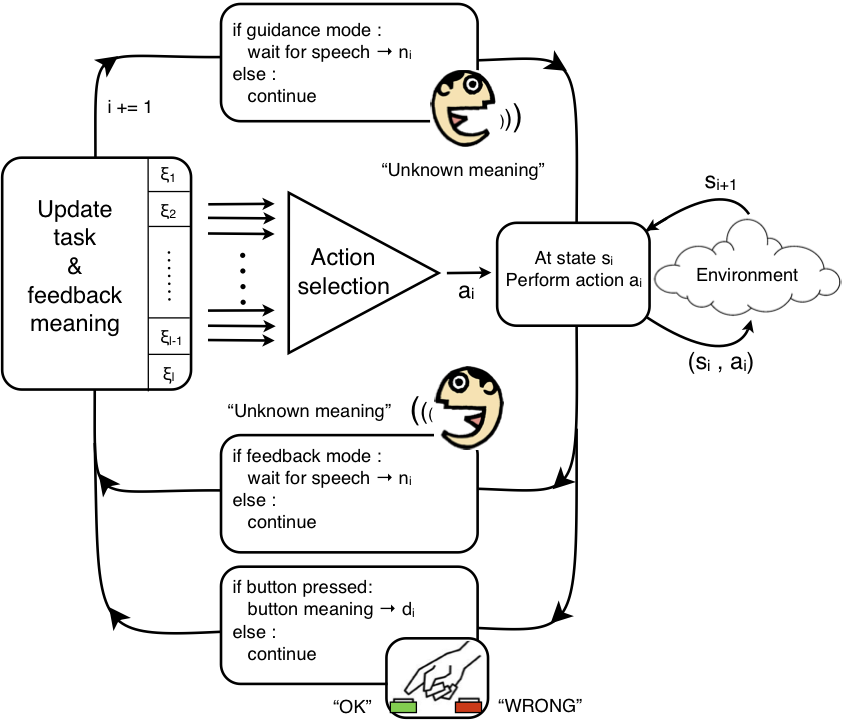
\includegraphics[width=0.6\columnwidth]{\imgpath/bloc.png}
  \caption{Experimental protocol showing the interaction between the teacher and the learning agent. The agent has to learn a task and the meaning of the instructions signals provided by the user, here recorded speech. The teacher can use guidance or feedback signals, and may also have access to buttons of known meanings for the robot.}
  \label{fig:lfui:bloc}    
\end{figure}

\subsection{Robotic System}

We consider a six d.o.f. robotic arm and gripper that is able to grasp, transport and release cubes in four positions. We used a total of three cubes that can form towers of at most two cubes.  The robot has 4 actions available: \textit{rotate left}, \textit{rotate right}, \textit{grasp cube} and \textit{release cube}. The state space is discrete and defined as the location of each object, including being on top of another object or in the robot's gripper. For a set of 3 objects we have 624 different states. Figure~\ref{fig:lfui:setup} shows the robot grasping the orange cube. 

\begin{figure}[!htbp]
  \centering
  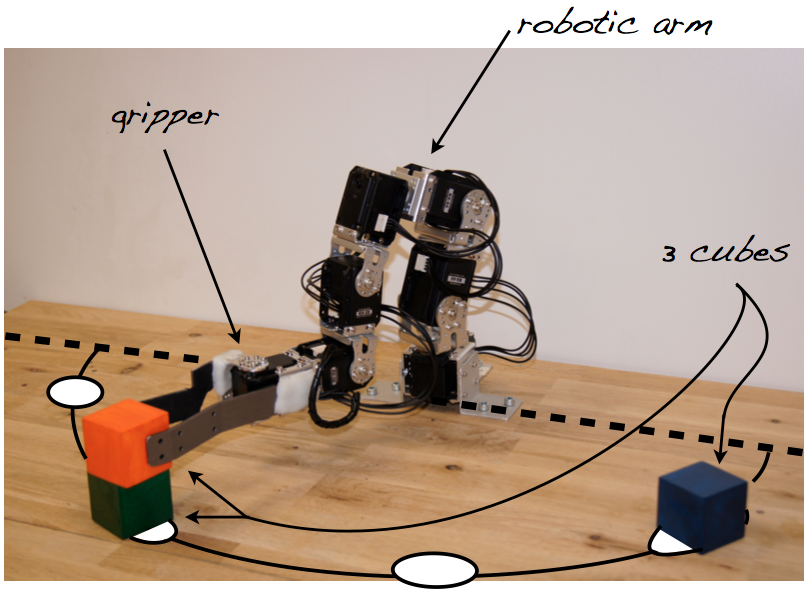
\includegraphics[width=0.5\columnwidth]{\imgpath/setup.png}
  \caption{The six d.o.f robotic arm and gripper learning to performing a pick-and-place task with three cubes.}
  \label{fig:lfui:setup}
\end{figure}

\subsection{Task Representation}

We assume that for a particular task $\xi$ we are able to compute a policy $\pi$ representing the optimal actions to perform in every state. One possibility is to use \textit{Markov Decision Processes} (MDP) to represent the problem \cite{sutton1998reinforcement}. From a given task $\xi$ represented as a reward function we can compute the corresponding policy using, for instance, Value Iteration \cite{sutton1998reinforcement}. In any case, our algorithm does not make any assumption about how tasks are represented.

For this particular representation, we assume that the reward function representing the task taught by the human teacher is sparse. In other words, the task is to reach one, yet unknown, of the 624 states of the MDP. Therefore we can generate possible tasks by sampling sparse reward functions consisting of a unitary reward in one state and no reward in all the other.

\subsection{Feedback and Guidance Model}
\label{chapter:lfui:framemodels}

From a given task $\xi$, we can compute the corresponding policy $\pi_{\xi}$. This policy allows to interpret the teaching signals with respect to the interaction protocol defined. In this experiment, we will consider the user is providing either feedback or guidance on the agent's actions. 

\paragraph{} For the feedback case, we define $p(l^f |s,a,\xi)$ as:
%
\begin{equation}
    p(l^f = \emph{correct} |s,a,\xi) = 
    \begin{cases}
    1-\alpha               & if~a = \argmax_a \pi_{\xi}(s,a)\\
        \alpha             & \text{otherwise}\\
   \end{cases}
   \label{eq:feedbackframe}
\end{equation}
%
with $\alpha$ modeling the expected error rate of the user and $p(l^f = wrong |s,a,\xi) = 1 - p(l^f = correct |s,a,\xi)$.

\paragraph{} For the guidance case, the user instructions represent the next action the robot should perform, therefore it only depends on the current state of the robot and the task considered. In our scenario, there is 4 different possible actions ($nA = 4$) in each state. We define $p(l^f |s, \xi)$ for each action as:
%
\begin{equation}
    p(l^f = a |s,\xi) = 
    \begin{cases}
        1-\alpha & if~a = \argmax_a \pi_{\xi}(s,a)\\
        \frac{\alpha}{nA-1} & \text{otherwise}\\
   \end{cases}
   \label{eq:guidanceframe}
\end{equation}
%
with $\alpha$ modeling the expected error rate and assuming only one action is optimal. As the agent can perform 4 different actions, we used the constant $\frac{\alpha}{3}$ for non-optimal actions in order to conserve the property that $\sum_a p(l^f = a |s,\xi) = 1$. For those cases where there is more than one optimal action, the probability is uniformly splitted among them. If all actions are optimal, they all share the same probability of $\frac{1}{nA}$.

\paragraph{} It is important to remember that these frames, while capturing a realistic interaction protocol, are arbitrary and we explicitly ask the users to conform to them. Here we assume that the teacher is aware of the optimal policies to fulfill the task, and additionally shares the same representation of the problem than the robot. Especially, for the scenario considered, the user should be aware that the robot can not move from position 1 to position 4 in one action. The robot should rather pass thought all intermediate positions $(1 \rightarrow 2 \rightarrow 3 \rightarrow 4)$. However as we known the user will sometime make teaching mistakes, we added a noise term $\alpha$ that account for unpredictable teaching mistakes. For all following experiments $\alpha$ was set to 0.1.

\subsection{Speech Processing}
\label{chapter:lfui:speechdata}

We consider speech as the modality for interacting with the robot. After each action we record the teaching word pronounced by the user. This data is mapped into a 20 dimensional feature space using the methodology described next.  

A classical method for representing sounds is the \textit{Mel-Frequency Cepstral Coefficients} (MFCC) \cite{zheng2001comparison}. It represents a sound as a time sequence of MFCC vectors of dimension 12. Comparing sounds is done via \textit{Dynamic Time Warping} (DTW) between two sequences of feature vectors \cite{sakoe1978dynamic}. This distance is a measure of similarity that takes into account possible insertions and deletions in the feature sequence and is adapted for comparing sounds of different lengths. Each recorded vocal signal is represented as its DTW distance to a base of 20 pre-defined spoken words which are \textbf{not} part of words used by the teacher.

By empirical tests on recorded speech samples, we estimate that a number of 20 bases words were sufficient and yet a relatively high number of dimensions to deal with a variety of people and speech. This base of 20 words has been randomly selected and is composed of the words:\emph{ \footnotesize{Error, Acquisition, Difficulties, Semantic, Track, Computer, Explored, Distribution, Century, Reinforcement, Almost, Language, Alone, Kinds, Humans, Axons, Primitives, Vision, Nature, Building}}.

% \subsection{Classification System for the Instruction Model}
\subsection{Classifiers}

Any machine learning algorithm working for classification problems can be used in our system. This classifier should be able to generalize from the data and should have appropriate underlying assumptions on the structure of those data. In other words, if the labels were known, the classifier should able to find a good mapping between the signals and their meanings. The only required characteristic is the ability to output a probability on the class prediction, i.e. $p(l|e, \theta)$.

In this study we decided to compare three classifiers:
\begin{itemize}
\item Gaussian Bayesian Classifier (also called quadratic discriminant analysis (QDA)): Computing the weighted mean $\mu$ and covariance matrix $\Sigma$, the usual equations for Gaussian mixture hold.
\item Support Vector Machine (SVM): Using a RBF kernel with $\sigma = 1000$ and $C = 0.1$. The parameter values have been estimated via a swap of parameters and by estimating performances via a cross validation procedure on the dataset. For SVM probabilistic prediction refer to \cite{platt1999probabilistic}.
\item Linear Logistic Regression: The predictive output value ($[0,1]$) is used as a probability measure.
\end{itemize}

Our classifier are tested on our labeled speech dataset in order to verify their adequacy to model the signal to meaning mapping. All three classifiers obtain accuracy close to 100 percent. This is a rather optimal scenario, we will see in next chapter~\ref{chapter:planning:results} how our algorithm behaves with data of poorer quality.

\subsection{Action selection methods}

% As different sampling methods can lead to different learning behaviors w

The selection of the robot's actions at runtime can be done in different ways. We will compare two different methods: random and  $\epsilon$-greedy. When following random action selection the robot does not use its current knowledge of the task and randomly selects actions. Whereas with $\epsilon$-greedy method the robot performs actions according to its current belief on the tasks, i.e. it follows the policy corresponding to the most likely task hypothesis. The corresponding optimal action is chosen with $1-\epsilon$ probability, otherwise, a random action is selected. In our experiment, we only consider results with $\epsilon =  0.1$.

It is only in the next chapter that we will investigate how the robot can actively selects its future actions in order to improve its performances.

\transition

Before presenting the results of our experiments, we illustrate in next section the pick and place scenario as well as the results of the labeling process for the feedback and guidance case.

%%%%%%%%%%%%%%%%%%%%%%%%%%%%%%%%%%%%%%%%%%%%%%
%%%%%%%%%%%%%%%%%%%%%%%%%%%%%%%%%%%%%%%%%%%%%%
%%%%%%%%%%%%%%%%%%%%%%%%%%%%%%%%%%%%%%%%%%%%%%
%%%%%%%%%%%%%%%%%%%%%%%%%%%%%%%%%%%%%%%%%%%%%%
%%%%%%%%%%%%%%%%%%%%%%%%%%%%%%%%%%%%%%%%%%%%%%
\section{Illustration of the pick and place scenario}
\label{appendix:pickplace}

We illustrate in Figure~\ref{fig:lfui:pickplaceworld} the pick and place world (where we used balls instead of cubes). There is three objects that can be moved in four different positions and stacked on two levels maximum. The robot's gripper can only grasp the object on top of the stack. An object is always released on top of a stack, except if the stack is full, in which case the release action produces no effect.

\begin{figure}[!htbp]
  \centering
  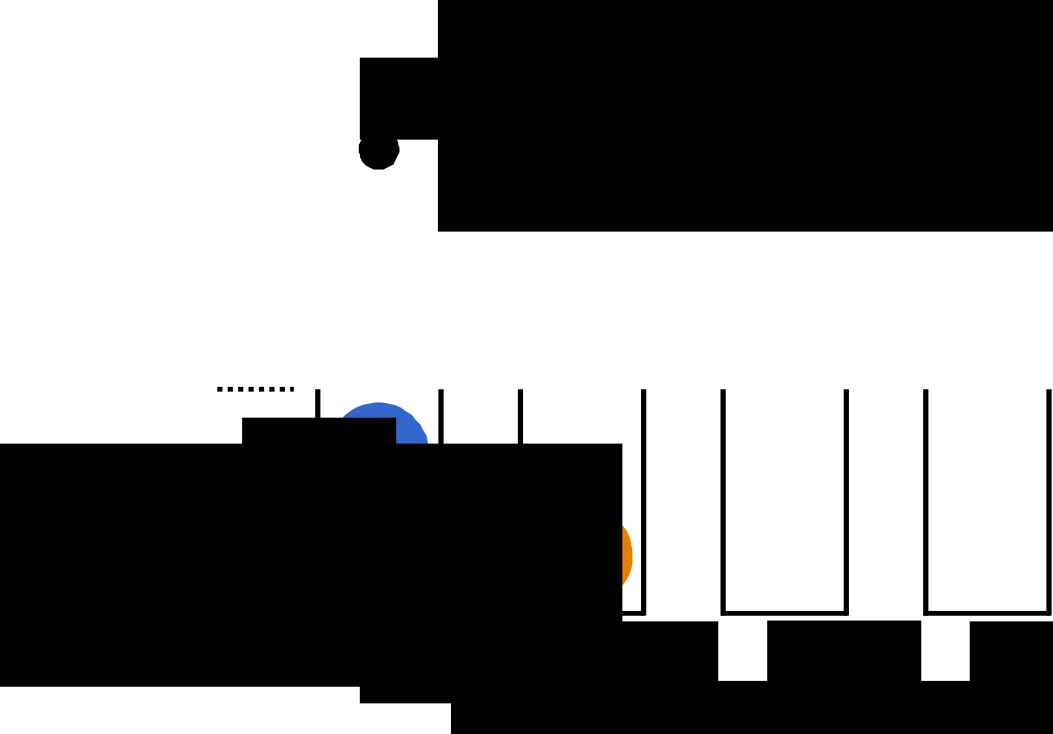
\includegraphics[width=\tworldsize\columnwidth]{\visualspdf/pick_and_place/pick_and_place_world.pdf}
  \caption{A schematic view of the pick and place problem. There is three objects that can be moved in four different positions and stacked on two levels maximum. The robot's gripper can only grasp the object on top of the stack. An object is always released on top of a stack, except if the stack is full, in which case the release action produces no effect.}
  \label{fig:lfui:pickplaceworld}
\end{figure}

In order to complete a task, i.e. to reach a specific configuration of cubes, the robot must perform an ordered sequence of actions. For illustration purpose, we only consider 3 out of the 624 possible hypotheses. Figure~\ref{fig:lfui:pickplacesequence} shows a sequence of actions starting in our hypothesis 1 configuration and going to our hypothesis 3 configuration using the shortest possible number of actions. Hypothesis 2 is a state on this path. While hypothesis 1 and hypothesis 3 seems ``close'' in terms of position of the cubes, they are actually ``far'' one from the other in terms of the action sequence.

\begin{figure}[!htbp]
  \centering
  \includegraphics[width=\columnwidth]{\visualspdf/pick_and_place/pick_and_place_sequence.pdf}
  \caption{A pick and place sequence showing three hypotheses and the sequence of actions from hypothesis 1 to hypothesis 3 through hypothesis 2. While hypothesis 1 and hypothesis 3 seems ``close'' in terms of position of the cubes, they are actually ``far'' one from the other in terms of the action sequence.}
  \label{fig:lfui:pickplacesequence}
\end{figure}

If the user is delivering feedback signals, the labeling process is presented in Figure~\ref{fig:lfui:pickplacefeedback} for a robot acting randomly in the environment. Note that hypothesis 1 and 2 are the most difficult to discriminate by acting randomly as they share most of their optimal policies.

\begin{figure}[!htbp]
  \centering
  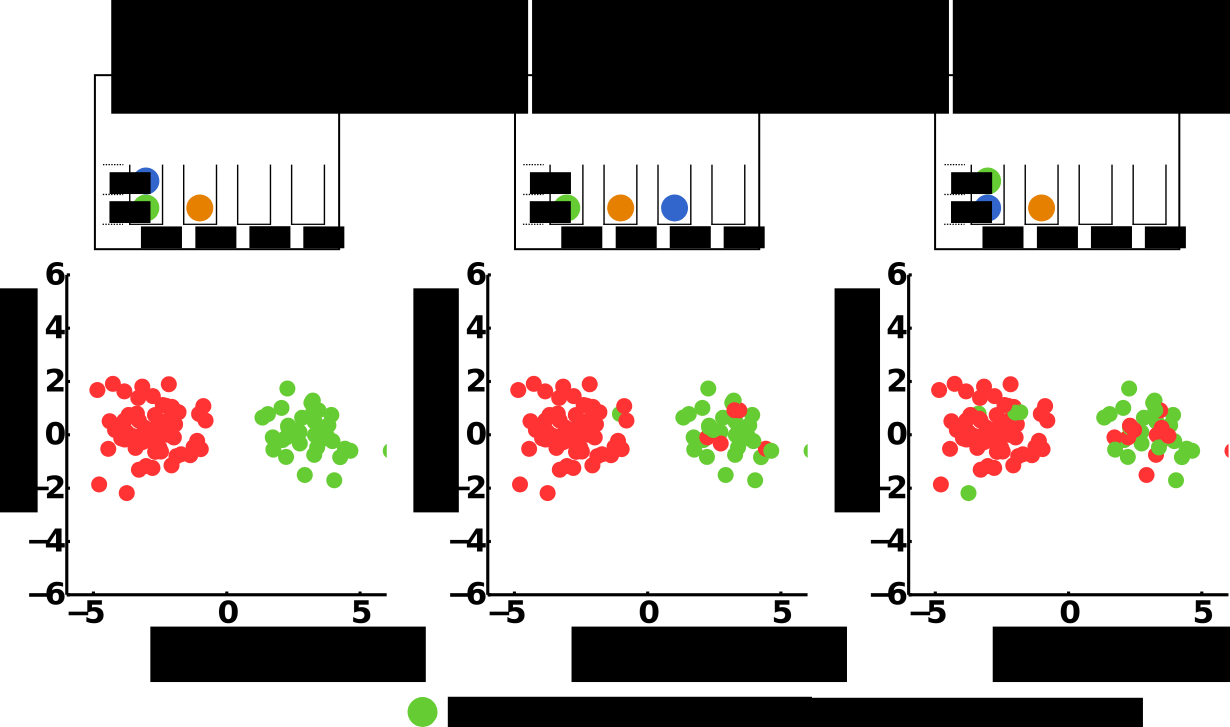
\includegraphics[width=\columnwidth]{\visualspdf/pick_and_place/pick_and_place_feedback.pdf}
  \caption{Results of the labeling process for our three hypotheses and considering the feedback frame. The robot explores randomly the state space. The teacher provides feedback with respect to hypothesis 1. Only a few state-action pairs allowed to differentiate between hypothesis 1 and 2.}
  \label{fig:lfui:pickplacefeedback}
\end{figure}

For the guidance case, the teacher uses the signals presented in Figure~\ref{fig:lfui:pickplaceguidancesignals} and the labeling process is presented in Figure~\ref{fig:lfui:pickplaceguidance} for a robot action randomly in the environment. Note that for some states there may be two optimal actions. For example, in Figure~\ref{fig:lfui:pickplacesequence}, for inverting two stacked cubes there is two different optimal policies, either the one presented in Figure~\ref{fig:lfui:pickplacesequence}, or putting the blue ball in position 2 and the green in position 3 during the exchange of position. These equally optimal options make the learning process more difficult, we can still visually find out that for hypothesis 1 all points in each cluster share one color, which is not the case for the other two hypotheses.

\begin{figure}[!htbp]
  \centering
  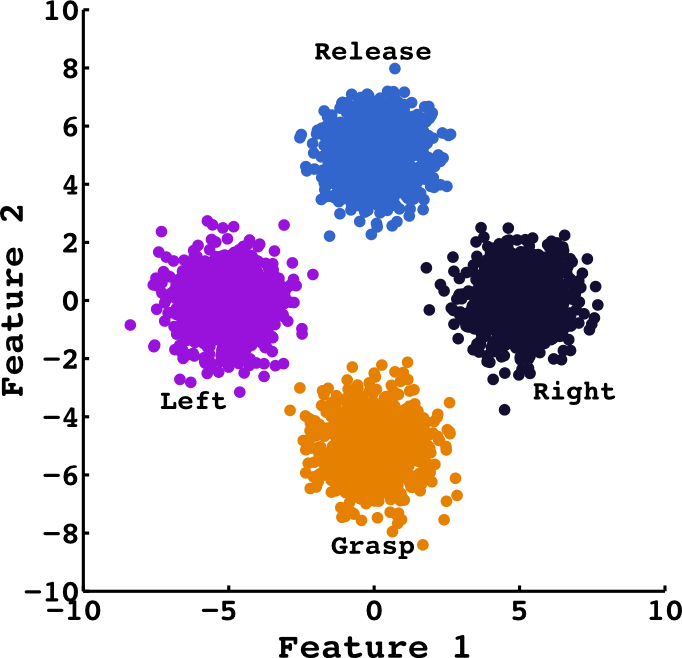
\includegraphics[width=\signalwidth\columnwidth]{\visualspdf/pick_and_place/guidance_pick_and_place.pdf}
  \caption{The guidance signals used for our visual example.}
  \label{fig:lfui:pickplaceguidancesignals}
\end{figure}

\begin{figure}[!htbp]
  \centering
  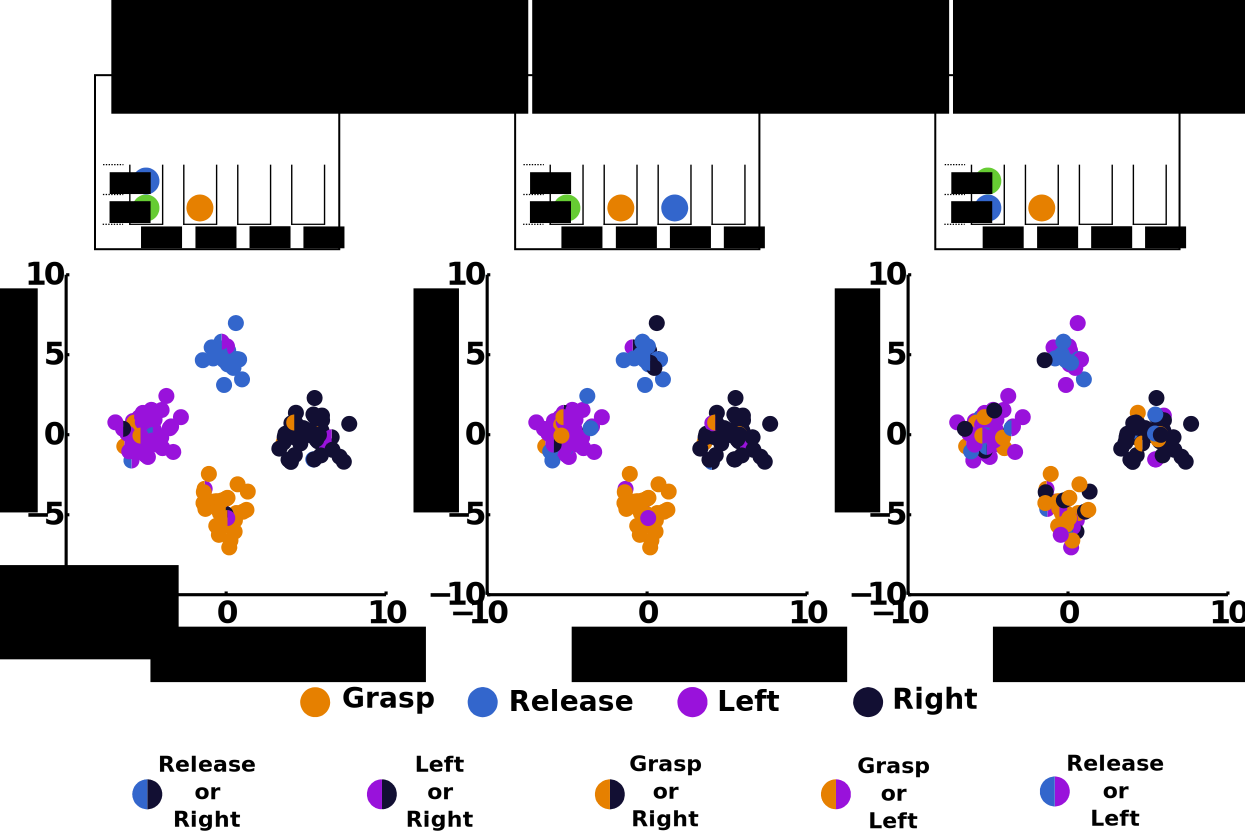
\includegraphics[width=\columnwidth]{\visualspdf/pick_and_place/pick_and_place_guidance.pdf}
  \caption{Results of the labeling process for our three hypotheses considering the guidance frame. The robot explores randomly the state space. The teacher provides guidance with respect to hypothesis 1. The labeled signals that contain two colors represent situations where the user could have given two different guidance signals, i.e. where two actions were optimal. It is only for hypothesis 1 that all signals in each cluster share one color. The case of guidance with multiple optimal actions in some states makes the learning process more ambiguous and may require some additional time compared to the feedback case.}
  \label{fig:lfui:pickplaceguidance}
\end{figure}

\transition

We have provided an example of the pick and place world with two dimensional signals and considering only three hypotheses. In next section, we consider real spoken words mapped to a 20 dimensional space and the full space of hypothesis which consists of 624 possible object configurations.

%%%%%%%%%%%%%%%%%%%%%%%%%%%%%%%%%%%%%%%%%%%%%%
%%%%%%%%%%%%%%%%%%%%%%%%%%%%%%%%%%%%%%%%%%%%%%
%%%%%%%%%%%%%%%%%%%%%%%%%%%%%%%%%%%%%%%%%%%%%%
%%%%%%%%%%%%%%%%%%%%%%%%%%%%%%%%%%%%%%%%%%%%%%
%%%%%%%%%%%%%%%%%%%%%%%%%%%%%%%%%%%%%%%%%%%%%%
\section{Results}
\label{chapter:lfui:results}

The experiments presented in this section follow the protocol described in figure~\ref{fig:lfui:bloc}, where each turn the agent performs one action and waits for the teaching signals from the teacher. We first present a set of simulated experiments using the same MDP as for the real world experiment. We start by assuming that the teacher provides feedback instructions without any mistakes. % , therefore only the noise inherent to the spoken signals remains. 
We compare first the different classifiers, and then the performances of $\epsilon$-greedy versus random action selection methods both for the feedback and guidance cases. Later, we present an empirical analysis of robustness to teaching mistakes. The last simulated experiment considers a teacher having also access to buttons of known meaning. Finally, we show a result using the real robot and a human user, where we study how signals knowledge learned in a first run can be used in a second one to learn more efficiently.

In order to be able to compute statistically significant results for the learning algorithm, we created a database of speech signals that can be used in simulated experiments. All results report averages of 20 executions of the algorithm with different start and goal states. 

As there is 624 hypotheses, we must update 624 likelihoods at each step. Depending on the likelihood equation considered this may not be feasible in real time. As our aim is to run our system in real time, and as we know that the speech signals in our dataset are well separated in their feature space, we use the simplest version of our likelihood estimation methods described in Equation~\ref{eq:matchingoverfitting}. To estimate the probability of each task we normalize the likelihood estimates $\L_(\xi_1),\ldots,\L_(\xi_T)$ to 1.

% The interested reader will find in appendix~\ref{appendix:pickplace} an illustration of the pick and place world as well as the results of the labeling process for the feedback and guidance case.

\subsection{Learning feedback signals}

In this experiment, the teacher is providing spoken signals whose meanings are either ``correct'' or ``incorrect''. The robot should simultaneously learn the task and the mapping between the spoken words and the binary meanings. The action selection of the robot is done using the $\epsilon$-greedy method. The user uses only one word per meaning.

The results comparing the different classification methods are shown in Figure~\ref{fig:FeedbackOneWord}. It shows the evolution of the probability associated to the task the teacher has in mind. We can track this information because we know, as experimenters, the true task taught by the teacher. Note that after 200 iterations all three classification methods identified the correct task as the most likely, i.e. the normalized likelihood values of the correct task are greater than 0.5, meaning that the sum of all the others is inferior to 0.5. Logistic regression provides the worse results in terms of convergence rate and variance.

\begin{figure}[!htbp]
  \centering
  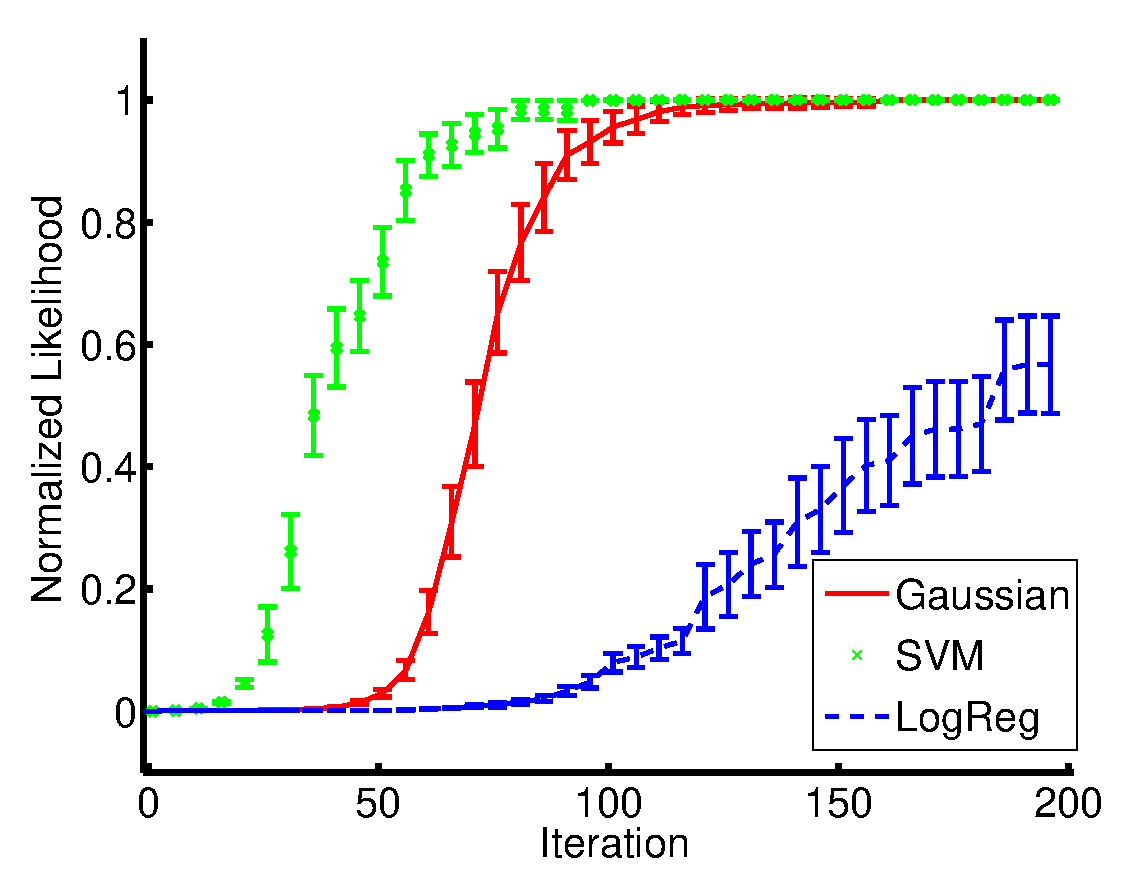
\includegraphics[width=0.7\columnwidth]{\imgpath/classifiers}
  \caption{Taught hypothesis normalized likelihood evolution (mean + standard error) thought iterations using different kinds of classifiers. The teacher is providing feedback signals using one word per meaning and the agent is performing actions according to the $\epsilon$-greedy strategy.}
  \label{fig:FeedbackOneWord}
\end{figure}

The user is not restricted to the use of only one word per meaning. Table~\ref{tab:1} compares the taught task normalized likelihood value after 100 iterations for feedback signals composed of one, three and six spoken words per meaning. SVMs have better performances when using one word per meaning but the Gaussian classifier has overall better results with less variance, see Table~\ref{tab:1}.

\begin{table}[!htbp]
\centering
\begin{tabular}{|l|c|c|c|}
\hline
&\textbf{One word}&\textbf{Three words}&\textbf{Six words}\\\hline
\textbf{Gaussian}&1.0 (0.1)&1.0 (0.1)&0.7 (0.1)\\\hline
\textbf{SVM}&1.0 (0.0)&0.5 (0.4)&0.3 (0.4)\\\hline
\textbf{LogReg}&0.1 (0.1)&0.2 (0.3)&0.2 (0.3)\\\hline
\end{tabular}
\caption{Taught hypothesis normalized likelihood values after 100 iterations (mean and standard deviation). Comparison for different classifiers and number of words per meaning. The Gaussian classifier has overall better performances.}
\label{tab:1}
\end{table}

Interestingly the Gaussian classifier learns better after 100 iterations than the other classifiers with many words per meaning. This counter intuitive result can be explain by the high dimensionality of the space where even one Gaussian can differentiate several groups of clusters. Linear logistic regression have lower performance presumably due to the linear decision boundary. For the SVM classifier, which is kernalized, as only 100 data points are distributed between each cluster, the more the number of clusters increases the less data points belong to each cluster. The fitting process of the SVM is therefore more likely to consider some data as noise, omitting some clusters. For the following experiments, we will only consider the Gaussian classifier, first because it has overall better performance, but also because it is the faster to train and thus is the only one usable for online experiments. 

% Indeed, in this setup, at each iteration the agent has to train 624 classifiers.

\subsection{Learning guidance signals}

In Figure~\ref{fig:Guidance}, we compare the performance between using feedback or guidance signals. From feedback to guidance the number of meanings is increased from two (correct/incorrect) to four (left/right/grasp/release). As depicted in Figure~\ref{fig:Guidance}, the robot is able to identify the task based on unlabeled guidance signals. However it requires more iterations to reach the same level of confidence. This may look counter intuitive because guidance signals are more informative. However the robot now needs to classify instructions in four different meanings, i.e. to identify four clusters of signals, which requires more samples. 

\begin{figure}[!htbp]
  \centering
  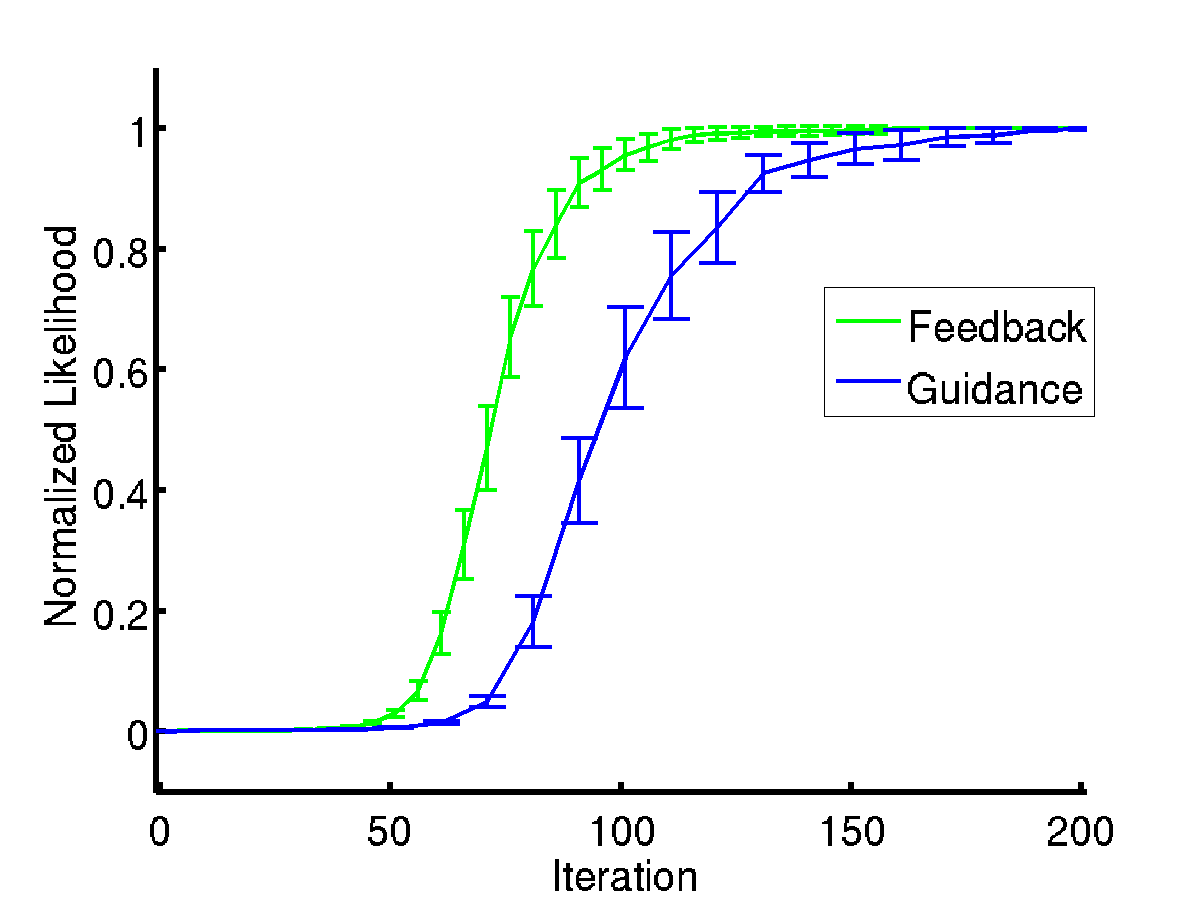
\includegraphics[width=0.7\columnwidth]{\imgpath/feedback_vs_guidance}
  \caption{Taught hypothesis normalized likelihood evolution (mean + standard error) thought iterations using Gaussian classifier. Comparison of feedback (green) and guidance (blue) instructions using one word per meaning. The robot is able to learn the task based on both feedback and guidance signals but needs more iterations for the guidance case.}
  \label{fig:Guidance}
\end{figure}

\subsection{Robustness to teaching mistakes}

Until now, we made the assumption that the teacher is providing feedback or guidance signals without any mistake. But in real world scenario, people can fail in providing optimal feedback. This is why we initially included the $alpha$ constant in our frame's equations (see section~\ref{chapter:lfui:framemodels}). An empirical analysis of robustness is shown in figure~\ref{fig:Noise} using feedback signals, Gaussian classifier, and one word per meaning. We compares two ways of training the Gaussian classifiers: \begin{inparaenum}[(1)] \item estimating the maximum likelihood (ML) of the Gaussian for each class, namely the mean and covariance, and \item using the expectation maximization (EM) algorithm \cite{dempster1977maximum} to iteratively update the mean and covariance of each class in order to find the underlying structure of the data. \end{inparaenum} 

% It allows to find the true underlying structure more efficiently.

We show that the EM approach is improving robustness to teaching mistakes. Referring to our previous discussion in section~\ref{chapter:lfui:whynotEM}, note that we initialized the EM algorithm with the ML estimates for each Gaussian, and we kept track which Gaussian belongs to which meaning. In addition, the representation used for the spoken words is of high quality and separates well the signals in the feature space. Therefore it is unlikely for the EM algorithm to fail at finding the two clusters given the data properties.

\begin{figure}[!htbp]
  \centering
  \begin{subfigure}[b]{0.49\columnwidth}
    \centering
    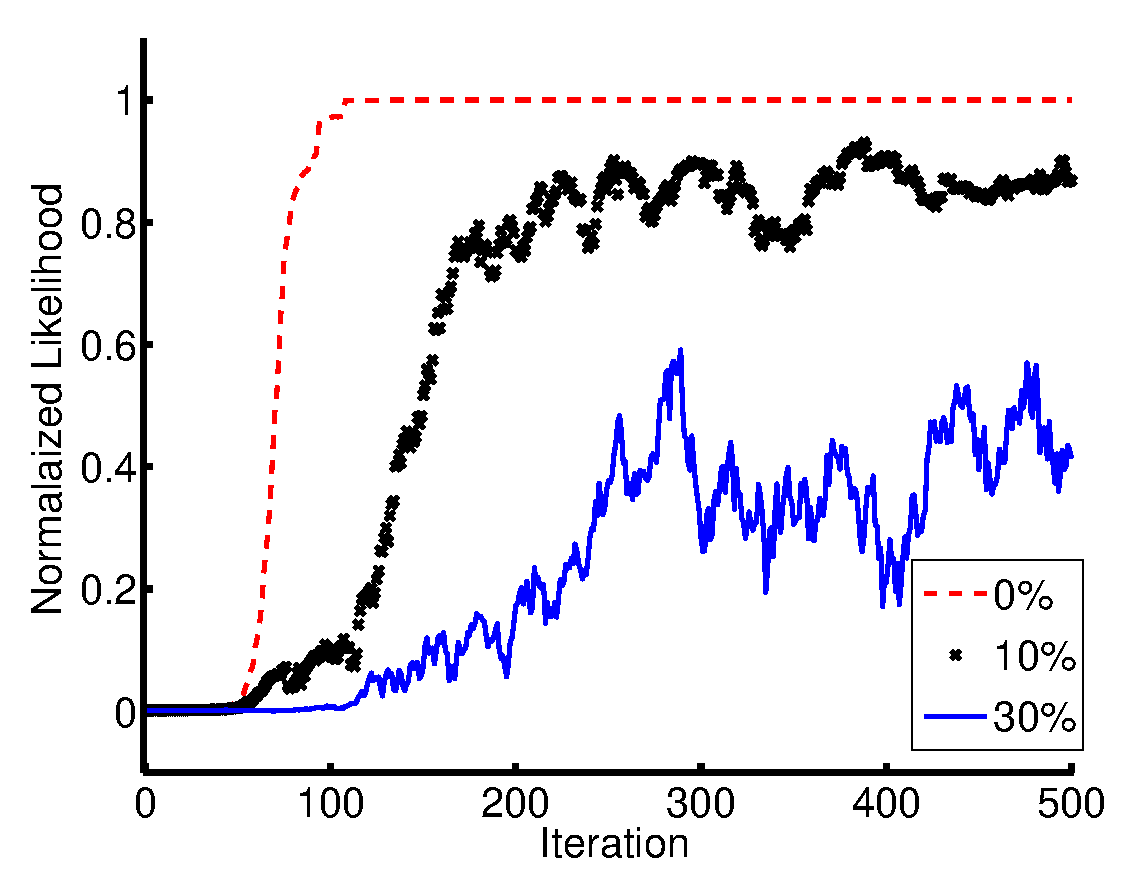
\includegraphics[width=\columnwidth]{\imgpath/noise_no_EM}
    \caption{ML}
  \end{subfigure}
  \begin{subfigure}[b]{0.49\columnwidth}
    \centering
    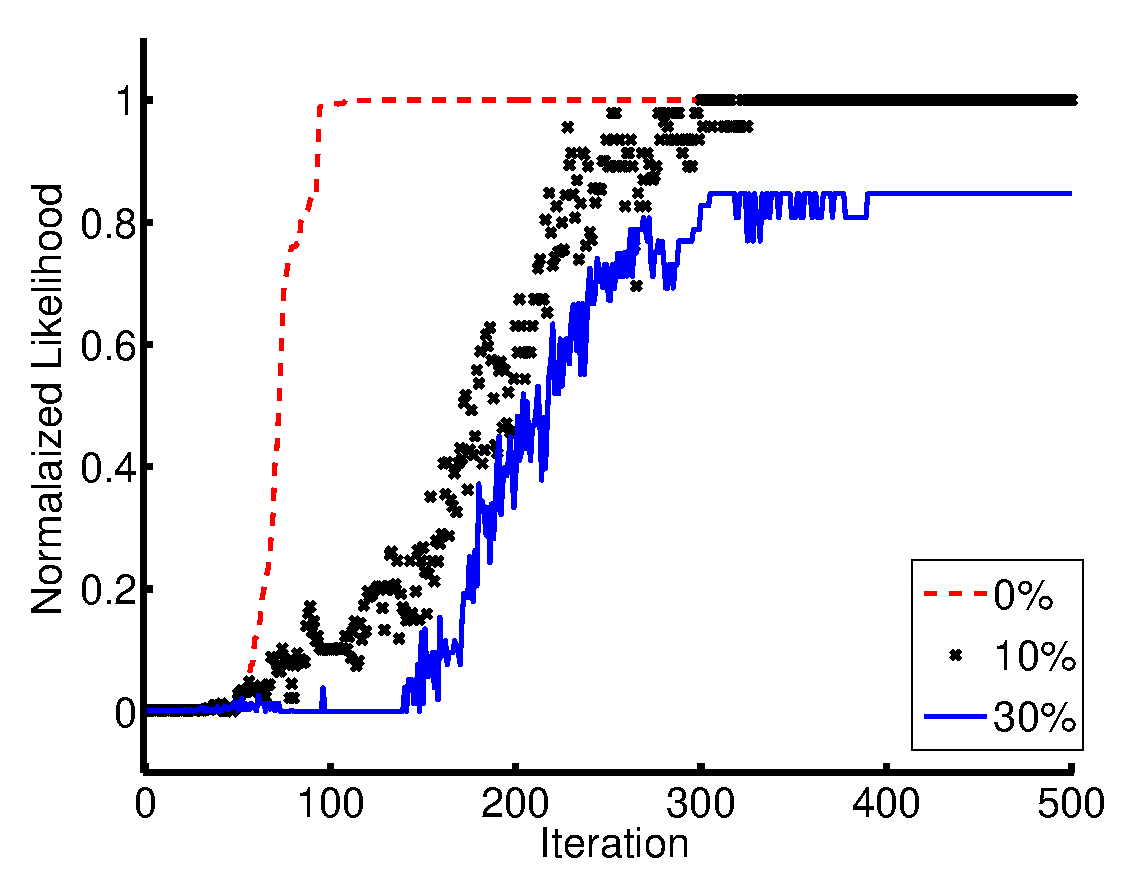
\includegraphics[width=\columnwidth]{\imgpath/noise_with_EM}
    \caption{EM}
  \end{subfigure}
  \caption{Taught hypothesis normalized likelihood evolution thought iterations using Gaussian classifier. Comparison of the ML estimates (left) versus EM estimates (right). The teacher is providing feedback using one word per meaning with different percentage of mistakes. Actions are selected following the $\epsilon$-greedy method. Standard error has been omitted for readability reason.}
  \label{fig:Noise}
\end{figure}

\subsection{Including prior information}
\label{sec:IncludingPriorInformation}

Learning purely from unknown teaching signals is challenging for the researcher but could be restrictive for the teacher. Therefore additional sources of known feedback are consider, such as a green and a red button, where the green button has a predefined association with a ``correct'' meaning, as red button with a ``incorrect'' meaning. 

% Yet, we shall expect that even in this case, users will use more modalities than the predefined one.

In this study, the teacher still provides unlabeled spoken words but can also use the red and green button as described in figure~\ref{fig:lfui:bloc}. However, and in order to avoid the possibility of direct button to signal association, the user can never use both modalities at the same time and use them alternatively with equal probability. Therefore, in average, after 250 iterations the robot has received 125 labeled button presses and 125 unlabeled speech signals. In most systems, the speech signals would be ignored but our method enables learning from the unlabeled signals. We compare three learning methods: \begin{inparaenum}[(1)] \item the robot is learning only via the labeled button presses, \item it uses only the unlabeled speech signals, and \item it uses both labeled and unlabeled signals. \end{inparaenum} Figure~\ref{fig:button} shows results from this setting. 

\begin{figure}[!htbp]
  \centering
  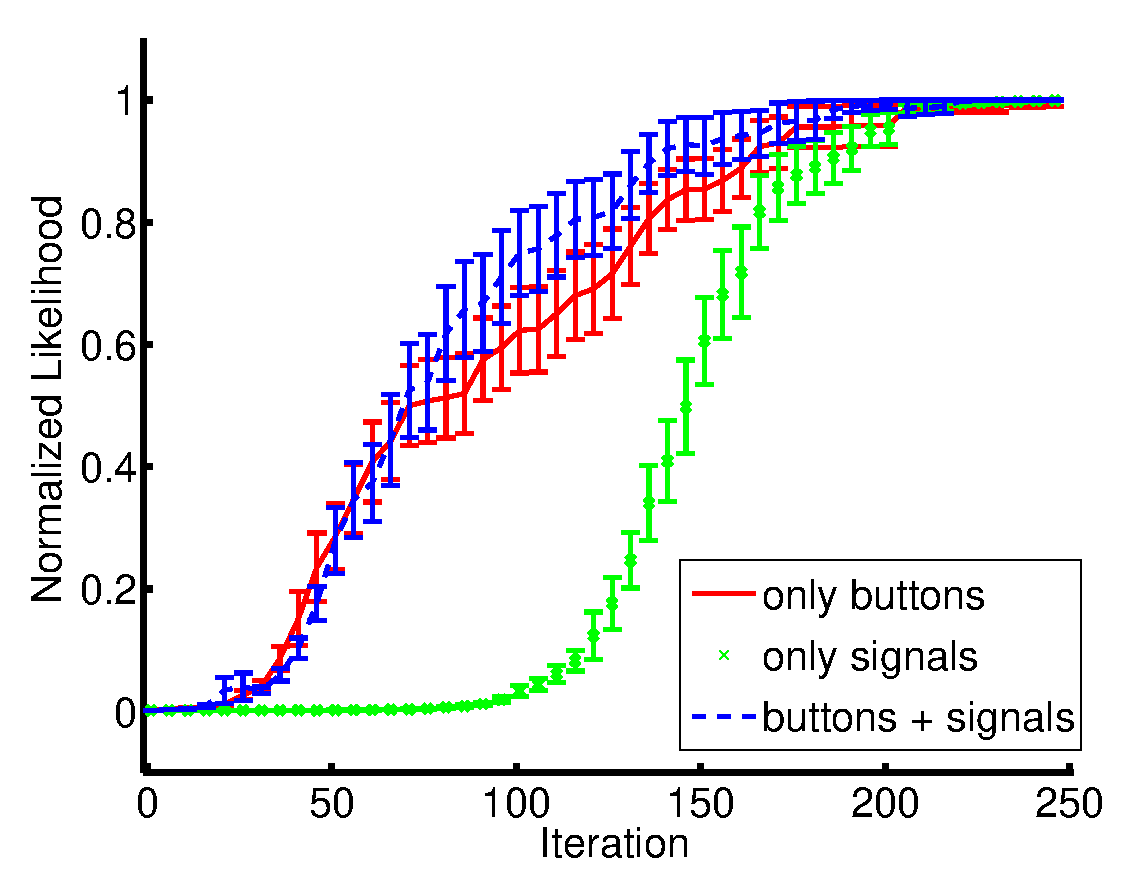
\includegraphics[width=0.7\columnwidth]{\imgpath/mix_button}
  \caption{Taught hypothesis normalized likelihood evolution (mean + standard error) thought iterations using Gaussian classifier. Comparison of using known button presses, unknown spoken signals, and both.}
  \label{fig:button}
\end{figure}

As expected, learning from labeled feedback is faster than with unlabeled signals. However taking advantage of different sources of information, even a priori unknown, can led to slightly better performances than using only known information. Importantly, the signals to meaning mapping of speech signals learned during a first task, could later be reused in further interactions.

\subsubsection{Reuse using a real robot}

Statistical simulations have shown that our algorithm allows an agent to learn a task from unlabeled feedback in a limited amount of interactions. To bridge the gap of simulation we tested our algorithm in real interaction conditions with our robotic arm. In this experiment, the teacher is facing the robot and chooses a specific goal to reach (i.e. a specific arrangement of cubes he wants the robot to build). He then decides one word to use as positive feedback and one as negative feedback, and starts teaching the robot. For this experiment the word \textit{``yes''} and \textit{``no''} were respectively used for the meaning ``correct'' and ``incorrect''. 

Once the first task has been identified by the robot, we keep in corresponding classifier and start a new experiment where the human teacher is going to use the same feedback signals to teach a new task. However the second time, the spoken words are first classified as ``correct'' or ``incorrect'' meaning according to the previously learned classifier. We study here two things, first does our system bridges the reality gap and can we reuse information about the signal to meaning mapping learned from a previous interaction session?

Figure~\ref{fig:Real} shows the result from this setting. In the first run it took about 100 iterations for the robot to identify the task. Whereas in the second run, when reusing knowledge from the first one, the robot is able to learn a new task faster, in about 30 iterations. The second run being faster that the first one indicates that our algorithm identified correctly the mapping between the user's speech signals and their corresponding meanings. 

The author of this thesis was the user for this studies and was therefore aware of the task representation used by the robot, i.e. a MDP with four discrete actions. As explained in chapter~\ref{chapter:related:humanintheloop}, an important challenge is to deal with non-expert humans whose teaching styles can vary considerably. While this challenge is not part of the current study, we observed that non-informed users teaching our robot had various understanding of the robot behaviors. It most often led to unsuccessful interactions due to an important amount of teaching mistakes from non-informed users.

% the two clusters in our $\mathbb{R}^{20}$ dimensional space as well as 

\begin{figure}[!htbp]
  \centering
  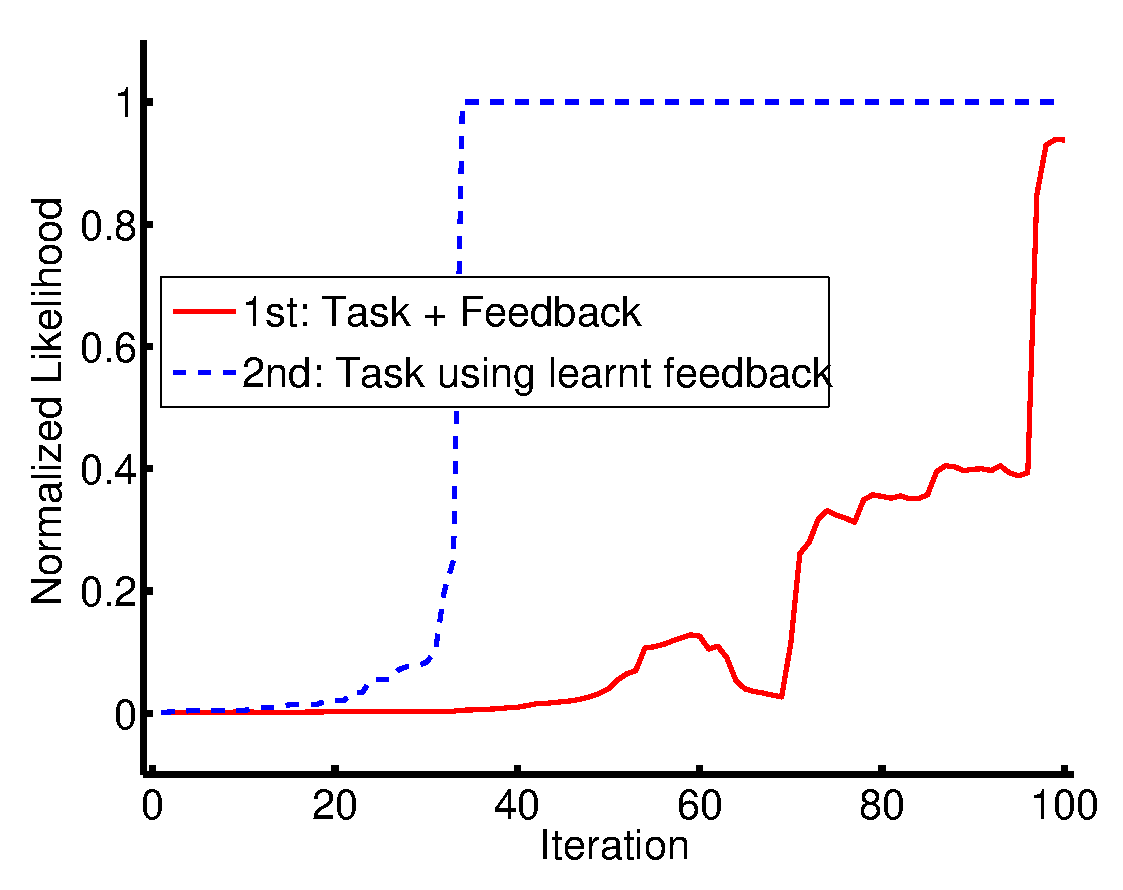
\includegraphics[width=0.7\columnwidth]{\imgpath/real}
  \caption{Taught hypothesis normalized likelihood evolution thought iterations using Gaussian classifier. A real teacher delivers spoken feedback signals using one word per meaning. The robot uses the $\epsilon$-greedy action selection method. A first run of 100 iterations is performed where the robot learns a task from unknown feedback. Then, by freezing the classifier corresponding to the most likely task, the user teaches the robot a new task.}
  \label{fig:Real}
\end{figure}

% We used a simplified version were the label from the first task are used to calibrate a classifier used for the learning of the second task.

\subsection{Action selection methods}

Finally, we compare the impact of using different action selection methods, we consider the $\epsilon$-greedy and the random action selection methods.

Figure~\ref{fig:selectionMethod} left and right compares respectively the action selection method for the case of feedback and guidance interaction frames. The $\epsilon$-greedy method results in a faster learning with less variance. The $\epsilon$-greedy method leads the robot in the direction of the most probable goal. In this way, the robot will receive more diverse feedback and will visit more relevant states than what a random exploration does.

\begin{figure}[!htbp]
  \centering
  \begin{subfigure}[b]{0.49\columnwidth}
    \centering
    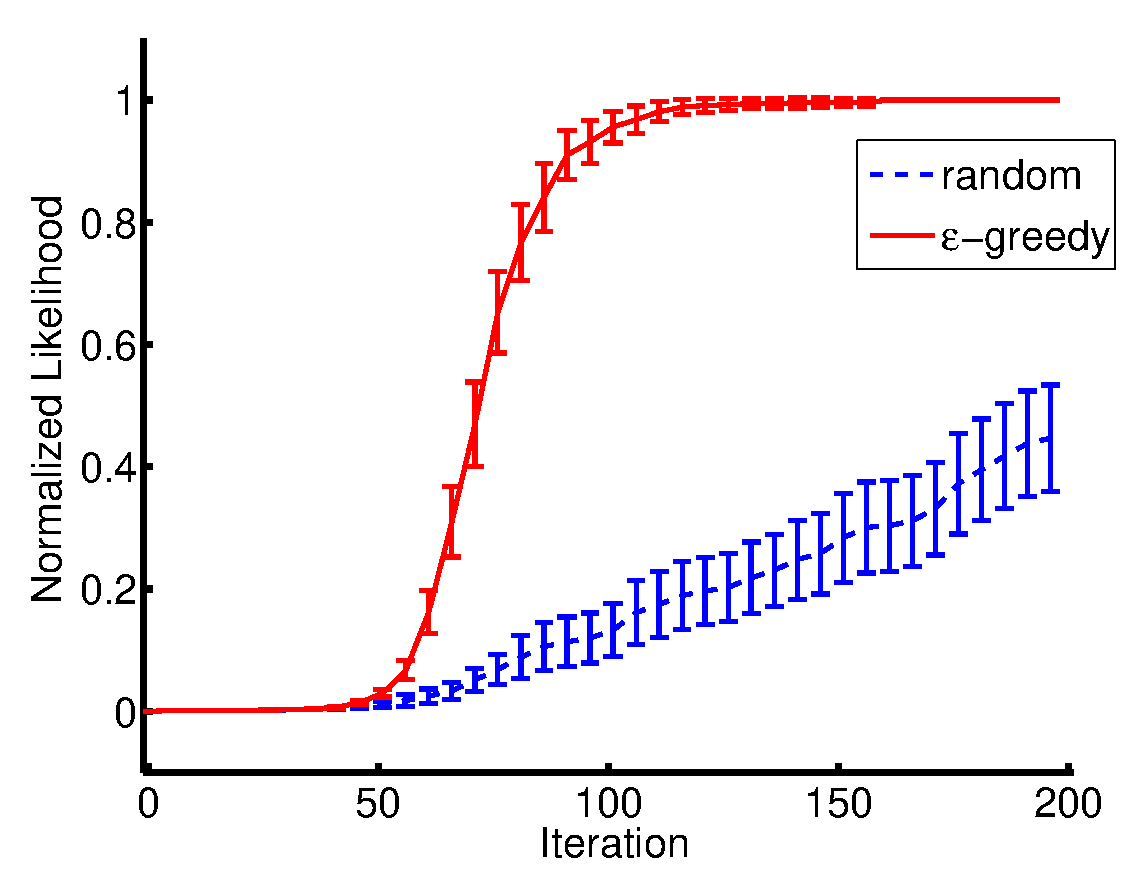
\includegraphics[width=\columnwidth]{\imgpath/feedback}
    \caption{Feedback}
  \end{subfigure}
  \begin{subfigure}[b]{0.49\columnwidth}
    \centering
    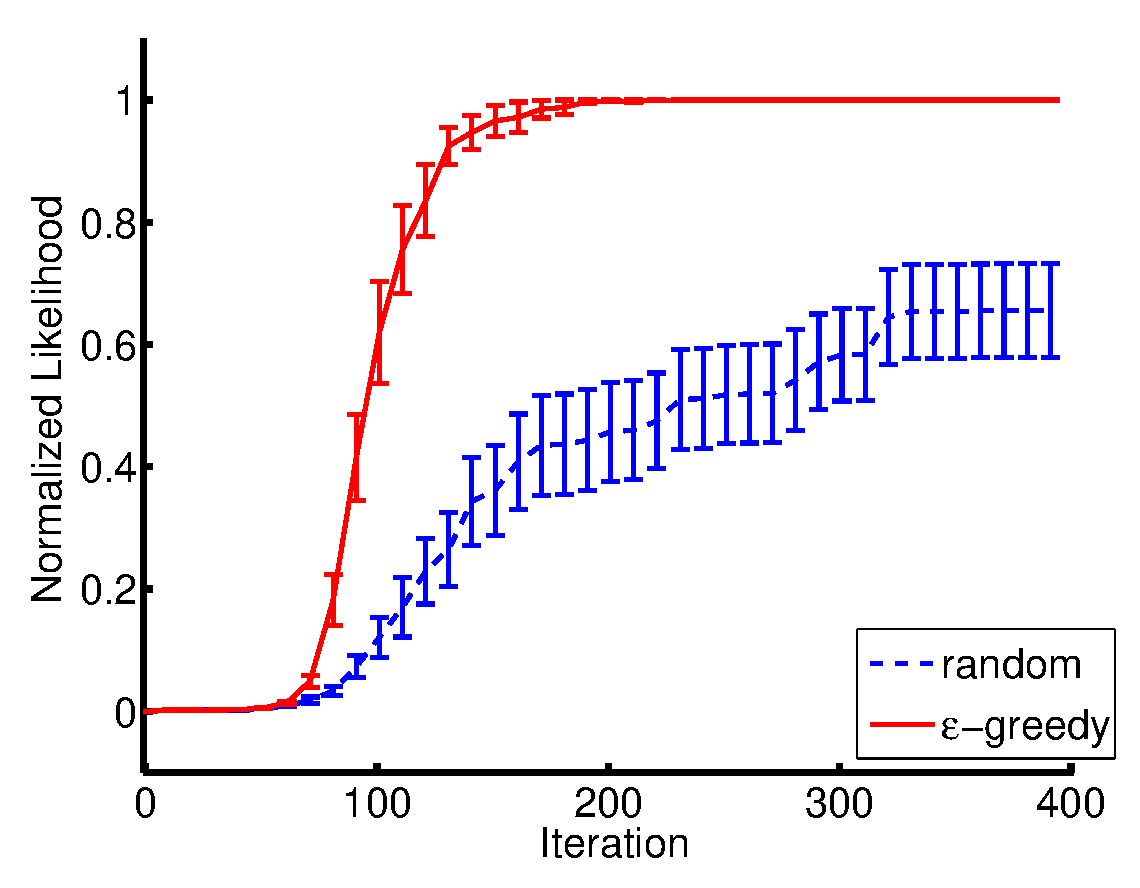
\includegraphics[width=\columnwidth]{\imgpath/guidance}
    \caption{Guidance}
  \end{subfigure}
  \caption{Taught hypothesis normalized likelihood evolution (mean + standard error) thought iterations using Gaussian classifier. The teacher is providing feedback (left) or guidance (right) signals using one word per meaning. The $\epsilon$-greedy action selection method allows a faster learning than the random method. Note that the x-axis, showing the number of iterations, does not considered the same range for the feedback (left) and guidance (right) cases.}
  \label{fig:selectionMethod}
\end{figure}

\transition

We showed that learning simultaneously a task and the meaning of an a priori unknown human instruction is possible and that the action selection method impacts the learning performances. Can we do better than random or $epsilon$-greedy action selection methods?

% This experiment was performed at a very early stage of this work and was not yet considering the full method introduced in section~\ref{chapter:lfui:tasttotask}.

Using an active learning approach \cite{settles2010active}, it might be more efficient to choose the actions that are expected to reduce the uncertainty as fast as possible. In next chapter, we investigate and details the specific properties of the uncertainty in our problem, where not only the task is unknown but also the signal to meaning mapping. We will provide measures of uncertainty that can be used as exploration bonuses for exploration strategies. We will finally present results from artificial dataset of different qualities in a two-dimensional grid world scenario.

%%%%%%%%%%%%%%%%%%%%%%%%%%%%%%%%%%%%%%%%%%%%%%
%%%%%%%%%%%%%%%%%%%%%%%%%%%%%%%%%%%%%%%%%%%%%%
%%%%%%%%%%%%%%%%%%%%%%%%%%%%%%%%%%%%%%%%%%%%%%
%%%%%%%%%%%%%%%%%%%%%%%%%%%%%%%%%%%%%%%%%%%%%%
%%%%%%%%%%%%%%%%%%%%%%%%%%%%%%%%%%%%%%%%%%%%%%
% \section{Discussion}

% In this work we presented an interactive learning system that can learn the initially unknown association between unlabeled instruction signals and their meaning while learning a new task. We presented empirical results showing that 1) our system can learn from unknown feedback, unknown guidance instruction signals, or a mixture of these signals, 2) it can recover from teaching mistakes, 3) it can leverage additional known sources of information, and 4) different standard classifiers can be used. An experiment with a real robot and a real user showed that 5) it can reuse acquired knowledge about human instruction signals in the learning of a new task. Finally we presented an extended experiment that mixed unknown feedback and guidance instructions, in a continuous environment, and showed that 6) an uncertainty based planning algorithm, using uncertainty from both task estimation and instruction classification, is the most efficient strategy.

% \subsection{Instruction modalities} Instruction signals were here conveyed using speech sounds (which may have been interjections, or even sounds of clapping or tapping hands). Of particular interest is the possibility to use the same system with multiple modalities for instruction signals, such as facial expressions or hand gestures. This allows different users to use the system according to their own modality preferences, potentially related to their own skills and limitations. In principle, since no part of the system is specific to the sound modality, and since the sound modality is already relatively complex, there are no theoretical obstacle for this experimental extension. An interesting example might be to consider brain-computer interfaces system \cite{chavarriaga2010learning, iturrate2010robot} that usually require a long an explicit training phase. Using our system we would be able to simultaneously understand the meaning of brain signals and what task is the user trying to achieve. We started investigating in that direction with promising preliminary results \cite{grizou2013zero}.


% say that the signal were very easy to classify




